\documentclass[a4paper,12pt]{article}  % sections, not chapters: a technical report

% Page layout
\usepackage[left=2.5cm,right=2.5cm,top=2.5cm,bottom=2.5cm]{geometry}

% Font and text
\usepackage[afrikaans,english]{babel}
\usepackage{microtype}
\usepackage{setspace}
\usepackage{lmodern}
\usepackage{siunitx}
\usepackage{tcolorbox}
% \usepackage[scaled=.96]{XCharter}
\usepackage[scaled=.96]{caladea}  % font required by Stellenbosch University
\usepackage[scaled=.96,lf]{carlito}  % the scaling makes the math the same height
\renewcommand*\oldstylenums[1]{\carlitoOsF #1}
\newcommand{\myemph}[1]{{\sffamily\bfseries#1}}
\sloppy
\onehalfspacing

% Headings
\usepackage[raggedright,sf,bf]{titlesec}
\usepackage[margin=\the\parindent,small,bf,sf]{caption}
\titlelabel{\thetitle.\ }
\makeatletter
\let\originall@section\l@section
\def\l@section#1#2{\originall@section{{\sffamily #1}}{#2}}
\makeatother

%% Alternative headings using small-caps (comment out the top section)
%\usepackage[raggedright,bf]{titlesec}
%\usepackage[margin=\the\parindent,small,bf]{caption}
%\titlelabel{\thetitle.\ }

% Table of contents
\let \savenumberline \numberline
\def \numberline#1{\savenumberline{#1.}}

% Figures
\usepackage{graphicx}
\usepackage{tikz}
\usetikzlibrary{arrows.meta,positioning,calc,backgrounds}
\usepackage{pdfpages}
\usepackage{subcaption}
\setlength{\abovecaptionskip}{7.5pt}  % spacing above and below captions
\counterwithin{figure}{section}
\newcommand*{\WaterMark}[2][0.2\paperwidth]{\AddToShipoutPicture*{\AtTextCenter{\parbox[c]{0pt}{\makebox[0pt][c]{\includegraphics[width=#1]{#2}}}}}}

% Mathematics
\usepackage[cmex10]{amsmath}
\usepackage{amssymb}
\usepackage{cancel}
\numberwithin{equation}{section}  % (3.1), as under the report class
\DeclareMathOperator*{\argmax}{arg\,max}
\newcommand{\T}{^\top}
\newcommand{\tr}{\textrm{tr}}
\renewcommand{\vec}[1]{\boldsymbol{\mathbf{#1}}}
\newcommand{\defeq}{\triangleq}

% Tables
\usepackage{booktabs}
\usepackage{tabularx}
\usepackage{longtable}  % tables that continue onto the next page (nomenclature)
\usepackage{xltabular}  % longtable with tabularx's X columns (appendix tables)
\usepackage{multirow}
\usepackage{float}  % [H]: place a table exactly where it is written
\newcommand{\mytable}{
    \centering
    \small
    \renewcommand{\arraystretch}{1.2}
    }
\renewcommand{\tabularxcolumn}[1]{m{#1}}
\numberwithin{table}{section}
\newcolumntype{C}{>{\centering\arraybackslash}X}
\newcolumntype{L}{>{\raggedright\arraybackslash}X}
\newcommand{\lowerbetter}{\ensuremath{\downarrow}}   % table header: lower is better
\newcommand{\higherbetter}{\ensuremath{\uparrow}}    % table header: higher is better

% Header and footer
\usepackage{fancyhdr}
\pagestyle{fancy}
\fancyhf{}
\renewcommand{\sectionmark}[1]{\markright{\normalsize \thesection.\ #1}}
\fancyhead[C]{\nouppercase{\textit{\rightmark}}}
\fancyhead[RO]{\thepage}
 \fancyhead[LE]{\thepage}  % double-sided printing
\fancyfoot{}
\setlength\headheight{14.5pt}
\renewcommand{\headrulewidth}{0pt}
\fancypagestyle{plain}{\fancyhead{}
                       \renewcommand{\headrulewidth}{0pt}
                       \fancyfoot[C]{\thepage}}

% Pseudo-code
\usepackage{algorithm}  % should go before \usepackage{hyperref}

% Table of contents and hyperlinks
\usepackage{hyperref}
\hypersetup{colorlinks=true,linktoc=all,citecolor=black,linkcolor=black}
\usepackage[nottoc]{tocbibind}
\addto\extrasenglish{%  % \autoref at every heading depth reads "Section"
  \def\sectionautorefname{Section}%
  \def\subsectionautorefname{Section}%
  \def\subsubsectionautorefname{Section}}

% Pseudo-code
\usepackage{algpseudocode}  % should go after \usepackage{hyperref}
\renewcommand{\thealgorithm}{\arabic{section}.\arabic{algorithm}}
\captionsetup[algorithm]{labelfont={bf,sf},font=small,labelsep=colon}

% Bibliography
\usepackage{cite}  % automatically reorder inline citations
\bibliographystyle{IEEEtran}

% Fix titlesec issue
\usepackage{etoolbox}
\makeatletter
\patchcmd{\ttlh@hang}{\parindent\z@}{\parindent\z@\leavevmode}{}{}
\patchcmd{\ttlh@hang}{\noindent}{}{}{}
\makeatother


\begin{document}

% Front matter
% Title page. TODO: confirm the exact degree wording and submission date with
% the department before submission.
\begin{titlepage}
\centering
\vspace*{2cm}

{\Huge\bfseries\sffamily Real-time Target Speaker Extraction\par}
\vspace{0.5cm}
{\Large\sffamily 
\par}

\vspace{2.5cm}
{\Large Grant Booysen\par}
\vspace{0.5cm}
{\large \texttt{25849646@sun.ac.za}\par}

\vfill
{\large
Thesis presented in partial fulfilment of the requirements for the degree of\\
% TODO: exact degree wording
\myemph{MSc in Machine Learning \& Artificial Intelligence}\\
in the Faculty of Science at Stellenbosch University\par}

\vspace{1.5cm}
{\large Supervisors: Dewald J. Swanevelder and David Botha (SmartOperator)\par}

\vspace{1cm}
{\large 
November 2026\par}
\end{titlepage}

\pagenumbering{roman}
% TODO: replace with Stellenbosch University's official declaration wording --
% do not paraphrase it, copy the current version from the faculty template.
\section*{Declaration}
\phantomsection
\addcontentsline{toc}{section}{Declaration}

By submitting this thesis electronically, I declare that the entirety of the work contained therein is my own, original work, that I am the sole author thereof (save to the extent explicitly otherwise stated), that reproduction and publication thereof by Stellenbosch University will not infringe any third party rights and that I have not previously in its entirety or in part submitted it for obtaining any qualification.

\vspace{2cm}
\noindent
\begin{tabular}{@{}p{6cm}p{1cm}p{6cm}@{}}
\textbf{Grant Booysen} & & \textbf{November 2026} \\
\hrulefill & & \hrulefill \\
Signature & & Date \\

\end{tabular}

\clearpage
\section*{Abstract}
\phantomsection
\addcontentsline{toc}{section}{Abstract}


\selectlanguage{english}

\clearpage
\section*{Acknowledgements}
\phantomsection
\addcontentsline{toc}{section}{Acknowledgements}

% TODO

\clearpage
\tableofcontents
\clearpage
%\listoffigures
%\listoftables
\section*{Nomenclature}
\phantomsection
\addcontentsline{toc}{section}{Nomenclature}

% Abbreviations used in the text. Add rows as they are introduced.
\subsection*{Abbreviations}
\begin{longtable}[l]{@{}ll@{}}
AMI & Augmented multi-party interaction \\
ASR  & Automatic speech recognition \\
BAK & Background intrusiveness (DNSMOS P.835 sub-score) \\
BSRNN & Band-split recurrent neural network \\
CARTSE & Li and Seki's online REAL-TSE system \cite{li2026cartse} \\
DNSMOS & Deep noise suppression mean opinion score \\
EQ & Equalisation \\
FR & Fabrication rate \\
GLU & Gated linear unit \\
ICR   & Interferer content rate \\
IHM & Individual headset microphone \\
ITU-T & ITU Telecommunication Standardization Sector \\
LAM & Large audio model \\
LCF-WER & Live-model content fidelity word error rate \\
LSTM  & Long short-term memory \\
LUFS & Loudness units relative to full scale \\
MLP & Multilayer perceptron \\
NLTK & Natural Language Toolkit \\
OVRL & Overall quality (DNSMOS P.835 sub-score) \\
REAL-TSE & Real-world target speaker extraction (challenge) \\
RIR & Room impulse response \\
RTF & Real-time factor \\
SAR & Signal-to-artefacts ratio \\
SDR & Signal-to-distortion ratio \\
SIG & Speech signal quality (DNSMOS P.835 sub-score) \\
SIR  & Signal-to-interference ratio \\
SI-SDR & Scale-invariant signal-to-distortion ratio \\
SLT & IEEE Workshop on Spoken Language Technology \\
SNR & Signal-to-noise ratio \\
STFT  & Short-time Fourier transform \\
TF Map & Time-frequency map \\
TSE   & Target speaker extraction \\
VAD & Voice activity detection \\
WER   & Word error rate \\
\end{longtable}



\subsection*{Symbols}

\subsubsection*{Signals and transcriptions}
\begin{longtable}[l]{@{}ll@{}}
$x$ & Mixture signal \\
$s$ & Target reference signal \\
$\hat{s}$ & Model output, the estimated target \\
$d$ & Interfering speech signal \\
$y_{(\cdot)}$ & Transcription of the subscripted signal \\
$y^\star_s$ & Ground-truth LibriSpeech transcription of the target \\
\end{longtable}

\subsubsection*{Model and objective}
\begin{longtable}[l]{@{}ll@{}}
$X$, $X_t$ & STFT of the mixture; frame $t$ of it \\
$X_e$, $x_e$ & STFT of the enrollment; the enrollment waveform \\
$S$, $\hat{S}$ & STFT of the target; of the model output \\
$\Re(\cdot)$, $\Im(\cdot)$ & Real and imaginary parts of a complex value \\
$N$, $H$, $h[n]$ & STFT window length, hop and window function \\
$\tilde{x}_t$, $\tilde{e}_j$ & Unit-length mixture frame; unit-length enrollment frame \\
$C_{t,j}$ & Cosine similarity of mixture frame $t$ and enrollment frame $j$ \\
$A_{t,j}$ & Softmax weight of enrollment frame $j$ for mixture frame $t$ \\
$\mu_t$, $u_t$ & Blended enrollment template; its unit-length direction \\
$m_t$, $\phi_t$ & Projection of $|X_t|$ onto $u_t$; the baseline cue $m_t u_t$ \\
$c_t$, $r_t$ & Similarity of $|X_t|$ to $u_t$; residual $|X_t| - m_t u_t$ \\
$M$, $R$ & Complex mask; residual spectrogram \\
$\alpha$, $s_\textup{proj}$ & Gain of the output along the target; $\alpha s$ \\
$e_\textup{int}$, $e_\textup{art}$ & Interference (other speaker and noise); artefact \\
% $d^{\perp}$, $e_d$ & $d$ with its target-like part removed; the part of $\hat{s}$ along $d^{\perp}$ \\  % REMOVED with the hail-mary loss, todo 2
$L_\textup{pres}$, $L_\textup{MR}$, $L_\textup{gain}$, $L_\textup{abs}$ & Loss terms \\
$w$, $w_\textup{m}$, $w_\textup{g}$ & Loss weights \\  % lambda removed with the hail-mary loss, todo 2
$\tau_\textup{pres}$, $\tau_\textup{abs}$ & Floors of $L_\textup{pres}$ ($10^{-3}$) and $L_\textup{abs}$ ($10^{-2}$) \\
\end{longtable}


\newpage
\pagenumbering{arabic}

% Contents
\section{Introduction}
\label{sec:introduction}
Voice assistants engage with users through direct, live speech-to-speech models such as Gemini Live \cite{google2026geminilive}. With the appearance of more voice based applications, the ability to engage with these tools in acoustically challenging environments is becoming increasingly important. A particular problem is the presence of interfering speech, which is misinterpreted by the live speech models as the intended target user speech. Interfering speech thus will confuse the downstream model as to the intended user input, which will lead to a poor user experience. Secondly, live speech models are exposed to noisy environments that include reverberation, background audio and other acoustic challenges. Although live models are fairly robust to background noise on its own (\autoref{sec:llms}), processing audio to remove interfering speech can introduce artefacts that the live model is not robust to. The work in this report aims to address these issues through the development of a target speaker extractor that aims to preprocess the audio input that is given to the live model. The extractor is constructed under the following constraints: it must be causal, process audio in real time and operate on a single channel of audio. However, an extractor can itself introduce artefacts that the live model hears as words, so it is not enough to measure whether the interfering speaker was removed; the evaluation must show which of the two errors the extractor causes.

Under these constraints, the contribution of this work lies not in a new architecture but in how the extractor is evaluated. The novel contributions are:
\begin{enumerate}
    \item \textbf{A live-model content fidelity evaluation suite.} The live model transcribes the extractor's output, and its errors are split into words leaked from the interfering speaker and words that neither speaker said (\autoref{sec:metrics}).
    \item \textbf{Evidence that the metrics are needed.} A single word error rate hides changes that the split reveals, and an offline transcriber misjudges changes that the live model does not notice (\autoref{sec:results}).
\end{enumerate}
To produce and test these, the following was built:
  \begin{enumerate}
    \setcounter{enumi}{2}
    \item \textbf{A constructed dataset and evaluation protocol.} \num{9955} training trials from \num{1172} LibriSpeech speakers, each rendered by constructing a simulated room with a random reverberation time and microphone and speaker positions, and then adding real background noise. Each speaker has exact transcripts. The dataset includes trials where the target is absent so that the extractor learns to stay silent (\autoref{sec:data}). 
    \item \textbf{A streaming target speaker extractor.} The REAL-TSE baseline architecture \cite{wang2026realtse}, implemented for this work and made fully causal, with the enrollment cue split into parts and a speaker embedding added (\autoref{sec:architecture}, \autoref{sec:e_architecture}). It runs in real time on a laptop CPU within the latency budget and reduces Gemini's word error rate from 53.3\,\% for the baseline to 39.6\,\%, while cutting the share of the interfering speaker's words that reach Gemini almost in half. On 123 held-out clips in which only the interfering speaker talks, it falls silent on 56 against 11 for WeSep, a larger offline system trained on different data, although WeSep recovers more of the target when both speakers talk (\autoref{sec:results_content_judge}).
    \item \textbf{A training loop with a proxy objective.} The live model cannot be differentiated through, thus the extractor is trained on a signal-level proxy objective adapted from CARTSE \cite{li2026cartse}.
  \end{enumerate}
  All results are for two-speaker mixtures and are optimised for Gemini.


The remainder of this report is structured as follows: \autoref{sec:litreview} reviews the background information and context for the target speaker extraction domain. \autoref{sec:methodology} describes the process of generating the data, the architecture of the extractor and the metrics. \autoref{sec:experiments} sets out how the model is trained, selected and evaluated. \autoref{sec:results} presents the results of the evaluation and \autoref{sec:conclusion} concludes the report with a summary and potential future work.
\section{Literature Review}
\label{sec:litreview}
The section presents and reviews target speaker extraction, streaming separation, how extraction is typically measured, and speech models as listeners. 
% TODO
\subsection{Target speaker extraction}
\label{sec:tse}

Target speaker extraction (TSE) is a well established task in speech processing. Meeting transcription systems, hearing aids, and smart speakers, these devices benefit from the ability for more robust speech recognition in the presence of background noise and competing speakers. The main idea is best described by Cherry's cocktail party problem \cite{cherry1953cocktail}. The problem is a description of a human's ability to focus on a single speaker in noisy environments, and using various indicators such as visual, spatial, and acoustic cues, can understand the speech of a target speaker while ignoring other speakers. The survey done by \v{Z}mol\'{i}kov\'{a} et al. \cite{zmolikova2023overview} provides a comprehensive overview, differentiating between three main tasks: target speaker extraction, blind source separation, and noise suppression. In this work, the focus is on target speaker extraction using only voice samples as an acoustic cue.

The intention behind the TSE task is to be able to deploy a system into a real-world scenario. However, due to the variability in the environments that a TSE system may be deployed in, a system must be robust to all conditions and listening scenarios. The survey by \v{Z}mol\'{i}kov\'{a} et al. \cite{zmolikova2023overview} highlights the gap that many TSE systems are not trained to go silent when the target speaker is not present, which is a separate task to extraction. The confound of the target speaker always present during training leaves the model vulnerable to situations where there is only interfering speech or noise. Another issue raised by \v{Z}mol\'{i}kov\'{a} et al. \cite{zmolikova2023overview} is that the use of signal level metrics such as signal-to-distortion ratio (SDR) is indicative of the ability of the model to extract speech, but \textit{(i)} it does not correlate with audible quality from the perspective of a human listener, and \textit{(ii)} it does not reflect the ability of the model to select or identify a target speaker as an evaluation metric. The survey also notes that TSE systems are being moved to low latency streaming setups. Therefore it is important to consider lightweight architectures that can be deployed in real-time scenarios. 

\subsection{Streaming separation}
\label{sec:streaming}
Separation models work with either a raw waveform or spectrogram. Some architectures such as Conv-TasNet \cite{luo2019convtasnet} favoured the waveform with the reasoning that calculating a spectrogram contributes to the latency of the system. However, Yu et al. adapted a Band-Split RNN (BSRNN) architecture, originally designed for music as an offline model \cite{luo2023music}, to speech enhancement tasks with an online configuration \cite{yu2023high}. Yu et al. found that their online implementation ran faster than real-time on an Intel i5 CPU.

TSE systems must work frame by frame, or chunk by chunk. The REAL-TSE challenge set a benchmark to say that a system must run with an algorithmic latency of \SI{100}{\milli\second} or less \cite{wang2026realtse}. Algorithmic latency, separate from end-to-end latency, is the delay built into the model: how long it must wait for audio before it can produce an output. The architecture must also be causal. For the REAL-TSE baseline this meant replacing bidirectional LSTMs over time with unidirectional ones. It also included normalising over a single frame or chunk rather than over the whole sequence \cite{wang2026realtse}. Claimed and measured latencies often disagreed in the challenge, so the organisers recommend reporting a component breakdown of the algorithmic latency.

A concern about streaming is that it makes it harder to identify the target speaker. As found in the survey by \v{Z}mol\'{i}kov\'{a} et al. \cite{zmolikova2023overview}, typical TSE systems use the entire context of an audio clip to identify the target speaker. However, in a streaming scenario, the system must identify the speaker quite quickly. The assumption in this work is that a \SIrange{200}{300}{\milli\second} end-to-end budget is sufficient. 

\subsection{How extraction is evaluated}
\label{sec:evaluation}
When making use of signal based metrics, practitioners are often required to use simulated data. This is because a clean reference signal is required for comparison against the model output. By nature it is quite difficult to obtain perfectly clean speech in a real-world scenario. Popular resources to use for simulated mixtures include Libri2Mix \cite{cosentino2020librimix} and WSJ0-2mix \cite{hershey2016deep}. Thus the first issue related to evaluation is the translation of performance on simulated data to real-world data. Zhang et al. \cite{zhang2021closing} show that there is not necessarily a direct translation in performance: in multi-channel speech enhancement, the model with the best signal-to-distortion ratio (SDR) on simulated data more than doubled its word error rate (WER) compared with the unprocessed input on real recordings from 19.5\,\% to 41.5\,\%. Signal scores also fail in the following manner for TSE: \textit{(i)} extracting a wrong speaker can still yield a low signal score due to similarities in speech, and \textit{(ii)} a silent target leaves the score undefined.

A natural guess to evaluate the performance of a TSE system is to suggest using perceptual metrics. These metrics are designed to mimic what a human listener would perceive when listening to the audio, for example DNSMOS \cite{reddy2021dnsmos}. However, as found by Wang et al. \cite{wang2026realtse}, these metrics can be gamed by adding adversarial perturbations to the waveform to inflate them. In other words, an extractor can be trained to maximise the perceptual metric without it improving the actual quality of the audio. Secondly, these perceptual metrics still fail in TSE as they do not identify if the wrong person is speaking.

The next progression would be to transcribe the audio and compare it against a ground truth transcription. The standard approach is to use the simple word error rate (WER) metric. However, this metric hides nuance in the failure of an extractor. Recognisers are hurt by the distortions of the extractor rather than by leftover noise left in the audio \cite{iwamoto2022bad} and secondly, a different recogniser may have different performance on the same audio. This leads into the shortcomings of WER as a metric for TSE. Suppose a word is heard from the interfering speaker, and secondly another word that neither speaker said and was invented, both can appear in the metric as a substitution or an insertion error. Finally the WER is only defined if there is target speech present.

\subsection{Speech LLMs as listeners and judges}
\label{sec:llms}
It is not a novel idea to make use of large language models (LLMs) to evaluate the quality of speech. In fact, Manakul et al. \cite{manakul2026audiojudge} found that large audio models (LAMs), which are LLMs that accept audio as input, are able to rank speech systems similarly to human raters. However, for tasks related to measuring speaking rate or speaker identity, the performance is poor and often close to random chance. The authors also found that these established LAMs that they tested are robust against noise and are more reliable on lexical content as opposed to non-lexical content.

Using a language model as a judge is a studied problem. Zheng et al.\ \cite{zheng2023judging} found that a strong text model can produce output that agreed with human preferences as often as humans agree with each other over 80\,\% of the time. However, a caveat to this is that the model's verdicts carried biases: it preferred the first option it was shown, longer answers, and output that it had generated itself. The concern is that the same biases may be present in audio models. A partial solution came from AIR-Bench \cite{yang2024airbench} that scores a pair of answers twice with the order reversed to prevent positional bias which is an idea carried through in the training of the model in this work where the target and interferer swap roles in an epoch to form two trials. Secondly, a model can leverage its prior knowledge of a language to make judgements instead of actually listening to the audio. This was explored by Foo et al.\ \cite{foo2026glitters} where audio language models keep 60--72\,\% of their benchmark scores even when the audio is removed. The prior was found to influence hallucination too as found by Koenecke et al.\ \cite{koenecke2024careless}. Another consideration is the handling of noisy audio. A natural response would be to enhance the audio first. However, enhancement was found to be detrimental according to Chondhekar et al.\ \cite{chondhekar2025denoising} where the denoising of medical speech actually raised the semantic WER of all four recognisers (including Gemini Flash 2.0) that were tested in 40 different configurations.

In Manakul et al. the study uses the model as a rater. The LAM is prompted for a verdict, such as preference over audio samples, and the final decision becomes the score. This work uses the model differently. The live model is only asked to write down what it heard and the score is computed by comparing the transcription to a ground truth text (Section~\ref{sec:lcfwer}). Each clip that is presented to the LLM is on its own, which mitigates positional bias that was found by Manakul et al. Their noise robustness was also only tested using white noise and did not explore competing speakers. Using the model as a listener rather than a rater is less common. The closest work reviewed here, Fela and Mowlaee \cite{fela2026perceptually}, found that standard audio-quality metrics fail to predict how often speech enhancement changes an LLM's downstream output. 

Therefore a gap remains. The studies making use of a model as a listener consider noise instead of competing speakers, and report a single error instead of a rate of error. None of the studies mentioned above consider the difference in error between a model leaking an interfering speaker versus inventing words that neither speaker said. This work proposes a measure to address this gap (\autoref{sec:lcfwer}).

\section{Methodology}
\label{sec:methodology}
The methodology section describes the process and reasoning behind the data generation, extractor architecture and evaluation metrics. 
% TODO
\section{Data construction}
\label{sec:data}
The section describes the construction of the dataset used for this work. It includes a description of the necessity of constructing the data from scratch, the source of the audio used, and the construction of the trials. 

\subsection{Why the data is constructed}
\label{sec:construct}
There are three main considerations for the dataset that need to be met: \textit{(i)} training requires a clean target signal as a reference for what the extractor should output, \textit{(ii)} the data must possess exact transcriptions of the target signal to allow for transcription-based evaluation, and \textit{(iii)} the data must possess both best case and worst case scenarios in order to interpret the performance of the extractor relative to these scenarios. These considerations limit the available choices of publically available datasets.

Constructing the data is also the established practice. The 2026 REAL-TSE challenge \cite{wang2026realtse} supplied no training set at all, and required that participants document whichever open-source data they used. The organisers after reviewing the submissions, describe the data recipe that the entrants converged on:

\begin{quote}
``Most teams synthesized mixtures from publicly available speech corpora such as LibriSpeech\ldots; added noise from WHAM!\ldots; and introduced reverberation with measured/simulated RIRs, while varying the number of speakers, SNR/SIR, RT60, chunk length, and enrollment quality. Many teams also injected target-absent or noise-only segments, forcing systems not only to extract the target when present but also to suppress non-target speech and avoid false extraction.''
\hfill\cite{wang2026realtse}
\end{quote}

The dataset constructed here follows that recipe, and the sections below describe each of its components in turn. The organisers further observed that several of the strongest entries were built on backbones near-identical to the official baseline architecture, the BSRNN, yet scored substantially better. They attribute the success to data simulation, real-data adaptation, pseudo-label filtering, loss design and post-processing rather than to architecture alone.    

\subsection{Source of audio}
\label{sec:audio}
The audio data was collected from a variety of sources to produce a diverse dataset. Speech was chosen for target and interferer from the LibriSpeech \cite{panayotov2015librispeech} dataset, which is a corpus of read English speech derived from audiobooks. The background noise was chosen from WHAM! \cite{wichern2019wham} which is a dataset of real-world noise recordings considering environments such as offices, streets, and cafés. 


\subsection{Trial construction}
\label{sec:trial_construction}
The trials are structured in a way to replicate the conditions of a real-world target speaker extraction scenario. Due to the difficulty of the TSE task, it was decided that the data should reflect a variety of conditions, but primarily focus on the base case task of a target speaker close to a recording device with an interfering speaker in a similar proximity and faint background noise. The difficulty came in constructing the dataset to be realistic enough to simulate a real-world scenario, but also not so difficult that a simple extractor of limited capacity would be unable to learn the task. A visual representation of the trial construction can be found in Figure \ref{fig:trial_construction}.
\begin{figure}[h]
    \centering
    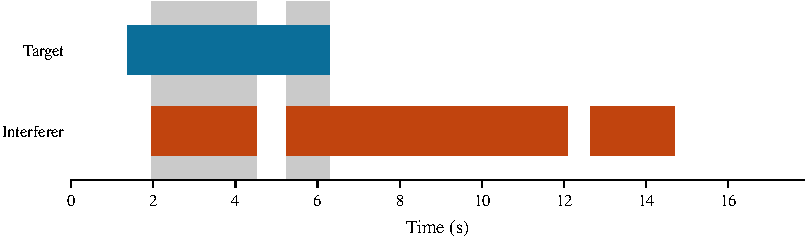
\includegraphics[width=0.7\textwidth]{figures/trial_timeline_low_overlap.pdf}
    \caption{Visual representation of the trial construction. The target and interferer are drawn from LibriSpeech, and the noise bed is drawn from WHAM!. The shaded areas show the overlapping regions of speech.}
    \label{fig:trial_construction}
\end{figure} 

A single trial consists of the following components: \textit{(i)} target speech, \textit{(ii)} interferer speech, \textit{(iii)} noise bed, \textit{(iv)} the mixture of the first three components, and \textit{(v)} an enrollment clip of the target speaker. The trial belongs to one of four conditions: both speakers present, only the target speaker present, only the interferer speaker present, and neither speaker present. The mixture is constructed to be 15-20 seconds long. The trials are drawn from two separate regimes: a base case and a difficult case. The base case is constructed to be a simple but realistic scenario, and difficult cases are edge cases that are constructed to be more challenging for the extractor. There are two both male and female speakers in the dataset. To simulate room acoustics, including reverberation, room dimensions, source and microphone positions, the \texttt{pyroomacoustics} \cite{scheibler2018pyroomacoustics} package is used to simulate the room impulse response. The trials are constructed to be as realistic as possible, but also to be reproducible and controllable. A sample of the room construction can be found in the Appendix \ref{sec:room_construction}. 

\paragraph{Enrollment.} [TODO validatae the enrollment clip length and whether it is a single clip or multiple clips]
The enrollment clip is a short audio segment of the target speaker. The clip is used to provide the extractor with a reference of what the target speaker sounds like. The clips are taken from the same source as the target speech, which is LibriSpeech. To avoid bias in the extractor, the enrollment clip is first attempted to be drawn from a different book reading. If this is unsuccessful, then the clip is drawn from a different chapter of the same book. Finally, if this is also unsuccessful, then the clip is drawn from a different utterance of the same chapter. The reason for this is to avoid the extractor memorising the target speech by learning to recognise the content rather than the \emph{manner} that the target speaker speaks. The distribution of enrollment clips across the dataset is shown in Figure \ref{fig:enrollment_distribution}. Again to avoid bias, the enrollment clips are simulated to come from different recording devices. This is done by applying equalisation (EQ) augmentation to the enrollment clips by applying a random EQ filter to the clip with a probability of \num{0.5}. This technique was suggested by the CARTSE \cite{li2026cartse} submission for the 2026 REAL-TSE challenge \cite{wang2026realtse}.
\begin{figure}[h]
    \centering
    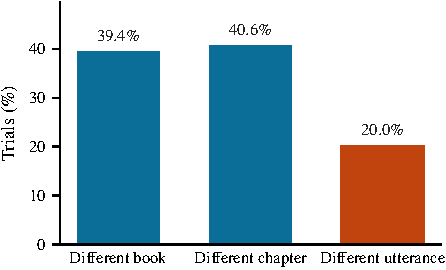
\includegraphics[width=0.7\textwidth]{figures/enrollment_provenance.pdf}
    \caption{Distribution of the source of the enrollment clips across the dataset.}
    \label{fig:enrollment_distribution}
\end{figure}


\paragraph{Parameter distribution choice.}
The Signal-to-Interference Ratio (SIR) is chosen uniformly from the range of -10 to 10 dB, and the Signal-to-Noise Ratio (SNR) is chosen uniformly from the range of 0 to 20 dB. These two ratios simulate the relative loudness of the target speaker to the interferer and background noise, respectively. A negative number for the SIR indicates that the interferer is louder than the target speaker, and the lower the SNR, the louder the background noise is relative to the target speaker. The SIR was chosen to be symmetric around \SI{0}{\decibel} after experimentation found that if the target was always (or majority of the time) louder than the interferer, then the extractor would just learn to follow the speech that was loudest and hence ignore the conditioning of the enrollment audio. This defeats the purpose of the task hence the stated requirement.

The reverberation of each room is set by a reverberation time, $T_{60}$, which is defined to be the time it takes for sound to decay by \SI{60}{\decibel}. The larger the value the more reverberant the room is. $T_{60}$ is drawn from a uniform distribution between \SIrange{0.25}{0.6}{\second}, which are values that span a carpeted office to a larger room with hard surfaces. To enforce realism, the absorption rate of the walls is also considered. The absorption rate is considered using the Sabine relation \cite{sabine1922}. The relation connects the physical properties of a room to its volume, its surface area and the absorption of its surfaces, so once the dimensions and the $T_{60}$ have been drawn the absorption is fixed by them and is solved for rather than sampled. A draw is rejected and replaced if the requested $T_{60}$ is not achievable in a room of the drawn size, which is also the reason for the lower bound of \SI{0.25}{\second}.

The remaining parameters and their distributions can be found in the Appendix \ref{app:params} 

\paragraph{Target-absent trials.} The extractor needs example trials to learn to rely on the conditioning of the enrollment audio to identify target speech. The target-absent trials support this idea by having the model learn to stay silent when the enrollment speaker is not present. The split is as follows for these trials: 49.5\% both speakers present, 25.5\% target only, 19.6\% interferer only and 5.4\% noise only.

\paragraph{Splits.} The dataset is split into a training and validation sets. Each of these sets have their own distinct set of speakers such that there is no overlap of speakers between the sets. The training set consists of \num{9955} trials, consisting of \num{1172} unique speakers. The idea behind this is to ensure that the model does not memorise speakers, but rather to learn to extract the target speaker based on the enrollment clip. The training split was progressively built up in stages from \num{1989} to \num{4976} and then finally to \num{9955} trials. This was done to measure the effect of the quantity of data on the performance of the extractor. The final evaluation holdout set consists of \num{200} trials of \num{40} unique speakers that is comprised of the following cases: \textit{(i)} 103 trials where both speakers are present, \textit{(ii)} 47 trials of the target speaker alone, \textit{(iii)} 42 trials of the interfering speaker alone and \textit{(iv)} 8 trials of neither speaker present.

\paragraph{Limitations.} The dataset is constructed to be as realistic as possible, but it is still a simulated dataset. The dataset is restricted to two speakers, which can confound the extractor to expect the target to be present if two speakers are present. Secondly, the combined audio forms \emph{read} speech and not \emph{conversational} speech. This means that the resulting audio does not have natural turn-taking, or conversational dynamics. These dynamics are simulated through the overlap of the target and interferer, but it is not a perfect simulation. Next, the dataset is restricted to English speech, and shoebox rooms only. Finally, the noise beds use are from WHAM! \cite{wichern2019wham} and range in length from 5 to 20 seconds long. This means that the noise beds are not long enough occassionally to cover the entire trial. To solve this, the noise bed is looped to cover the entire trial. 


\subsection{Baseline model architecture}
\label{sec:architecture}
The baseline architecture section describes the architecture that was used as a backbone in the REAL-TSE baseline \cite{wang2026realtse}. The architecture in this work is built from scratch, but the design is that of the baseline.
% Block diagram of the extractor as implemented. Drawn for this work.
% Provenance is stated per component in the caption, not wholesale: the diagram
% is not a redraw of any published figure -- the causal time path and the third
% input channel do not appear in one.
%
% Requires, in the preamble: \usetikzlibrary{arrows.meta,positioning,calc,backgrounds}
\begin{figure}[htbp]
\centering
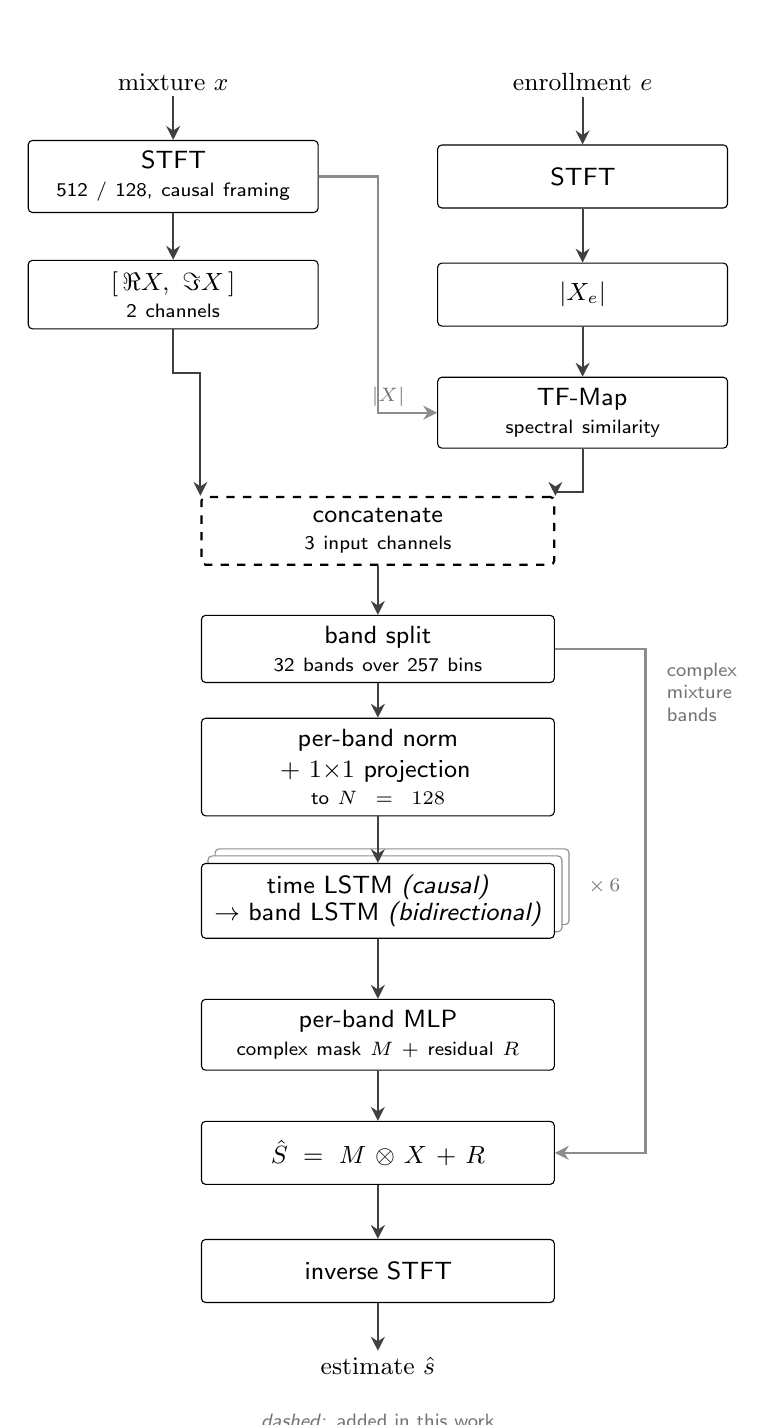
\begin{tikzpicture}[
    font=\small\sffamily,
    >={Stealth[width=5pt,length=5pt]},
    block/.style={draw, fill=white, rounded corners=1.5pt, align=center, inner sep=4pt,
                  minimum height=8mm, text width=42mm},
    inblock/.style={block, text width=34mm},
    ours/.style={block, dashed, thick},
    sig/.style={font=\small, inner sep=2pt},
    note/.style={font=\scriptsize\sffamily, text=black!55},
    arr/.style={->, thick, black!75},
    skip/.style={->, thick, black!45}
  ]

  % ---------- inputs -------------------------------------------------------
  % Columns sit symmetrically about the trunk at x = 3.5 and are narrower than
  % the trunk blocks, so the upper half does not overhang it.
  \node[sig] (xin) at (0.9,0) {mixture $x$};
  \node[sig] (ein) at (6.1,0) {enrollment $e$};

  \node[inblock] (stft1) at (0.9,-1.2) {STFT\\[-1pt] \scriptsize 512 / 128, causal framing};
  \node[inblock] (stft2) at (6.1,-1.2) {STFT};

  \node[inblock] (ri)  at (0.9,-2.7) {$[\,\Re X,\ \Im X\,]$\\[-1pt] \scriptsize 2 channels};
  \node[inblock] (mag) at (6.1,-2.7) {$|X_e|$};

  \node[inblock] (tfmap) at (6.1,-4.2) {TF-Map\\[-1pt] \scriptsize spectral similarity};

  \node[ours] (cat) at (3.5,-5.7) {concatenate\\[-1pt] \scriptsize 3 input channels};

  % ---------- trunk --------------------------------------------------------
  \node[block] (split) at (3.5,-7.2)  {band split\\[-1pt] \scriptsize 32 bands over 257 bins};
  \node[block] (norm)  at (3.5,-8.7)  {per-band norm $+$ $1{\times}1$ projection\\[-1pt] \scriptsize to $N=128$};
  \node[block] (bsnet) at (3.5,-10.4) {time LSTM \emph{(causal)}\\[-1pt] $\to$ band LSTM \emph{(bidirectional)}};
  \node[block] (est)   at (3.5,-12.1) {per-band MLP\\[-1pt] \scriptsize complex mask $M$ $+$ residual $R$};
  \node[block] (apply) at (3.5,-13.6) {$\hat{S} = M \otimes X + R$};
  \node[block] (istft) at (3.5,-15.1) {inverse STFT};
  \node[sig]   (out)   at (3.5,-16.3) {estimate $\hat{s}$};

  % Six identical blocks, drawn as a stack rather than annotated with an arrow:
  % offset copies on the background layer sit behind the front block.
  \begin{pgfonlayer}{background}
    \foreach \d in {0.18,0.09}{
      \draw[draw=black!45, fill=white, rounded corners=1.5pt]
        ($(bsnet.south west)+(\d,\d)$) rectangle ($(bsnet.north east)+(\d,\d)$);
    }
  \end{pgfonlayer}
  \node[note, anchor=west] at ($(bsnet.north east)+(0.30,-0.30)$) {$\times\,6$};

  % ---------- signal flow --------------------------------------------------
  \draw[arr] (xin) -- (stft1);
  \draw[arr] (ein) -- (stft2);
  \draw[arr] (stft1) -- (ri);
  \draw[arr] (stft2) -- (mag);
  \draw[arr] (mag) -- (tfmap);
  \draw[arr] (ri.south)    -- ++(0,-0.55) -| (cat.north west);
  \draw[arr] (tfmap.south) -- ++(0,-0.55) -| (cat.north east);
  \draw[arr] (cat) -- (split);
  \draw[arr] (split) -- (norm);
  \draw[arr] (norm) -- (bsnet);
  \draw[arr] (bsnet) -- (est);
  \draw[arr] (est) -- (apply);
  \draw[arr] (apply) -- (istft);
  \draw[arr] (istft) -- (out);

  % TF-Map needs the MIXTURE magnitude as well as the enrollment's. Label sits on
  % the segment entering TF-Map, not back at the STFT it leaves.
  \draw[skip] (stft1.east) -- ++(0.75,0) |- (tfmap.west);
  \node[note] at ($(tfmap.west)+(-0.62,0.20)$) {$|X|$};

  % The complex mixture bypasses the network: the mask multiplies into it, not
  % into the network's features.
  \draw[skip] (split.east) -- ++(1.15,0) |- (apply.east);
  \node[note, align=left, anchor=west] at ($(split.east)+(1.30,-0.55)$)
        {complex\\mixture\\bands};

  % ---------- legend -------------------------------------------------------
  \node[note] at (3.5,-17.0) {\emph{dashed}: added in this work};

\end{tikzpicture}
\caption{The extractor as implemented. Band splitting and the interleaved
band-level and sequence-level modelling follow \cite{luo2023music}; the
mask-plus-residual estimator follows \cite{yu2023high}; TF-Map conditioning
follows \cite{zhang2025multi}. The causal time path and the third input channel
are this work's.}
\label{fig:baseline-architecture}
\end{figure}

\subsubsection{Band-split Recurrent Neural Network (BSRNN)}
\label{sec:bsrnn}
Luo and Yu \cite{luo2023music} propose the BSRNN model as a frequency-domain separation model that is designed for high sample rate audio, in which the input audio is transformed from its waveform representation into a time-frequency representation using the Short-Time Fourier Transform (STFT). The model then divides the input spectrum into multiple frequency bands that are modelled independently. The original use case for the BSRNN model is music source separation, but in this work, the model is adapted to allow for the extraction of a target speaker from a mixture of speech signals. The development from music source separation to the method of the target speaker extraction (TSE) approach that this work follows came from the following lineage: \textit{(i)} music source separation was adapted to personalised speech enhancement (PSE) by Yu et al. \cite{yu2023high}. The authors proposed target speaker extraction in the PSE task by appending a target speaker enrollment module that was designed to suppress any interference. PSE can be summarised as enrollment-conditioned extraction. \textit{(ii)} Zhang et al. followed this framework and proposed a new module for the enrollment conditioning module, namely the Time-Frequency Map (TF Map) \cite{zhang2025multi}.


\subsubsection{Short-time Fourier transform}
\label{sec:stft}
The model operates in the time-frequency domain rather than a waveform. To ensure the input audio is in suitable form, a short-time Fourier transform (STFT) is applied by cutting the waveform into short, overlapping frames. A window function is applied to each frame, and then a discrete Fourier transform is applied to each windowed frame. The result is a complex-valued spectrogram, a two-dimensional representation of the audio signal. On the horizontal axis is time, and on the vertical axis is frequency. The discrete Fourier transform is defined as:
\begin{equation}
X(f, t) = \sum_{n=0}^{N-1} x[tH + n]\,h[n]\,e^{-\mathrm{j}2\pi fn/N},
\label{eq:stft}
\end{equation}
 where $N$ is the window length, $H$ the hop between frames, $h[n]$ a Hann window and $\mathrm{j}$ the imaginary unit. Following Yu et al.\ \cite{yu2023high}, $N = 512$ and $H = 128$ at \SI{16}{\kHz}: a \SI{32}{\ms} window moving in \SI{8}{\ms} steps, giving 257 frequency bins. Frames are not centred on timestamps as this would imply future information which is not suitable for streaming tasks. Instead, the signal is padded with $N - H$ samples at the start of a sequence.


\subsubsection{Band plan}
\label{sec:bandplan}

The spectrogram of Section~\ref{sec:stft} has 257 outputted frequency bins, each covering an equal slice of \SI{31.25}{\Hz}. However, each band should be modelled independently. Most of the structure that distinguishes one voice from another sits at the lower frequencies: the pitch of a voice and the resonances that give a vowel its identity all fall below about \SI{4}{\kHz}, and energy falls away steadily above that. The bins near the top carry far less information and thus would be wasteful to model with the same level of detail as the bins near the bottom.  

A band plan is the decision of how to group those bins. Bins are gathered into bands and each band is then handled separately by the network: it gets its own normalisation and projection. This allows a band to be compared against itself over time rather than against the loud low-frequency bands next to it. Grouping few bins per band keeps fine detail. Secondly grouping many bins into one band summarises coarsely but costs far less. A band plan therefore decides where the model's resolution is spent. 

 The plan in this work divides the 257 bins into 32 bands: fifteen of 3 bins (about \SI{100}{\Hz}) up to \SI{1.4}{\kHz}, ten of 6 bins (about \SI{200}{\Hz}) up to \SI{3.3}{\kHz}, five of 16 bins (\SI{500}{\Hz}) up to \SI{5.8}{\kHz}, one of 64 bins (\SI{2}{\kHz}) up to \SI{7.8}{\kHz}, and a final band of the 8 remaining bins at the top of the spectrum. Figure~\ref{fig:bandplan} shows it against a real mixture in the training set. This plan follows the implementation from Zhang et al.\ \cite{zhang2025multi} for their \SI{16}{\kHz} target speaker extraction model and used by the challenge baseline built on it, but no reason is given for these particular boundaries, and no explanation is given in previous papers.

\begin{figure}[htbp]
\centering
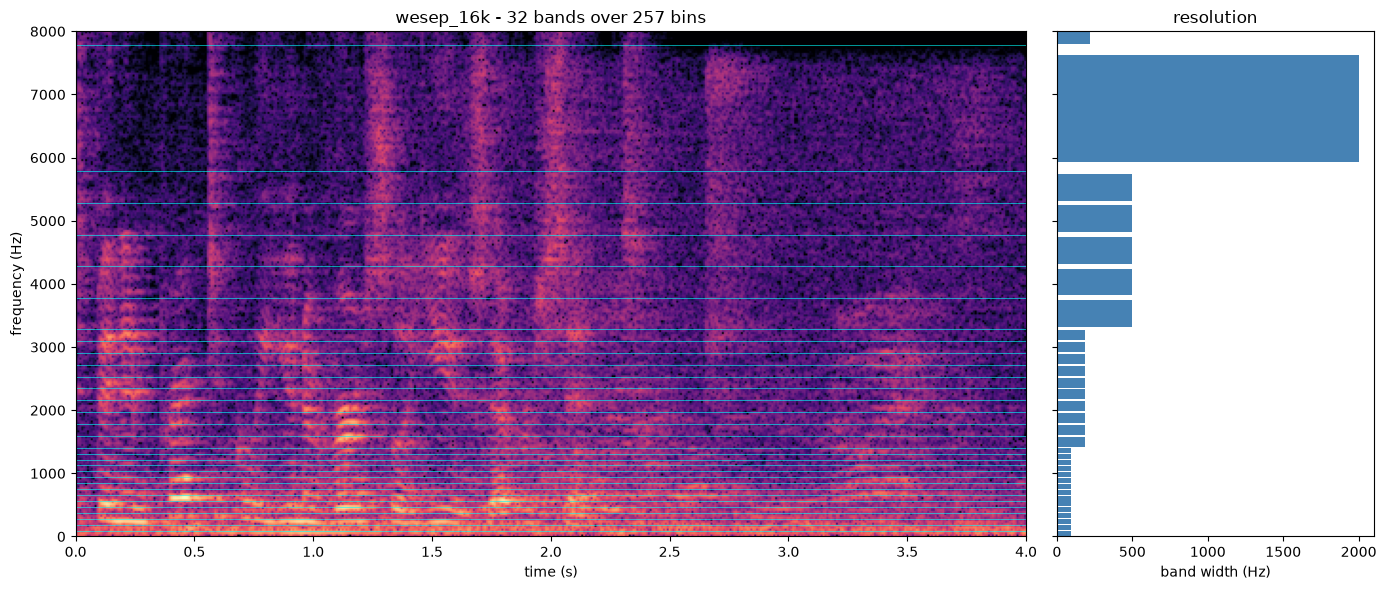
\includegraphics[width=\textwidth]{figures/bandplan-wesep.png}
\caption{The band plan used here, shown against a four-second mixture from the training set. Left: the band boundaries drawn over the spectrogram, closely spaced at the bottom where the speech structure is and widening upwards. Right: the width of each band in hertz.}
\label{fig:bandplan}
\end{figure}


\subsubsection{Per-band normalisation}
\label{sec:subbandnorm}

The bands defined by Section~\ref{sec:bandplan} are not comparable with one another. Each band typically carries different amounts of energy; therefore, if all 257 bins were scaled together, there would be a severe imbalance. The high bands would be underrepresented and thus diluted, effectively reducing the model's ability to learn the high-frequency features. Giving each band its own scaling is what prevents that. A band at \SI{6}{\kHz} is then judged against its own typical level rather than against the bands beneath it.

Following \cite{yu2023high} the approach first normalises the band, using a layer normalisation applied across the channels of that band. Secondly, because the bands must be the same size before they can be stacked together, a projection is required to map the band to a fixed width. Since there are varying sized and independent bands, each band has its own projection, which is a learnable linear layer that maps the band to a fixed width of 128 values. Every band is given the same structure but its own weights, so nothing is shared between bands and each is free to learn a representation suited to its own frequency range. The result is a stack of 32 bands, each with 128 features, which is then passed to the next module.

Normalisation is applied across the values of a band \emph{within a single frame}. Each frame is therefore normalised using only itself. This is a deliberate design choice that \emph{opposes} Yu et al.\ \cite{yu2023high}, who use batch normalisation for their online configuration. The opposition is for the following reasons: \textit{(i)} during training, the mean and variance are computed from the current batch, but during inference, these statistics are computed from the entire training set. The function that is optimised during training is therefore not the function that is deployed. \textit{(ii)} The variability of the data does not give a reliable estimate of the true distribution. The statistics of a batch therefore depend on what was drawn, and a silent crop normalised alongside loud ones is not normalised as it would be at inference. \textit{(iii)} Single frame normalisation carries no state and is unaffected by the amount of audio processed, so a four-second training chunk is normalised exactly as a stream that has been running for a minute.


\subsubsection{Residual LSTM block}
\label{sec:resrnn}

Two kinds of sequential structures are modelled: time and frequency. Time is unidirectional, but frequency is bidirectional, as all of the bands of a frame are available at the same instant and can be traversed in either direction. The block is used for both kinds of modelling, with the same structure but different parameters.

At inference time, since the model is running in a streaming fashion, the LSTM's internal state is preserved between frames and information can be carried forward indefinitely. The LSTM is therefore a natural fit for the task, and it is used in the same way for both the time and frequency sequences.

The block is made of three steps applied in order, following \cite{luo2023music}. The input is first normalised, then passed through the LSTM, and the LSTM's output is then mapped back to the input's width by a learned projection. The final addition is a residual connection and is inspired by the original ResNet \cite{he2016deep} architecture. This allows the gradient an unobstructed path back through the computation stack of all the blocks, which matters because six of these blocks are stacked in Section~\ref{sec:bsnet}. This is important as the LSTM is a deep recurrent layer, and the gradient can vanish or explode as it passes through the LSTM's internal state. The residual connection allows the gradient to bypass the LSTM entirely, which is what allows the model to train when the gradient vanishes within the LSTM. 

A single LSTM layer is given a width of 192, which is Yu et al.'s \cite{yu2023high} choice for their \SI{16}{\kHz} model. The input to the block is 128 wide, which is projected to 192 for the LSTM and then projected back to 128 for the residual addition. 

\subsubsection{Band and sequence model}
\label{sec:bsnet}

The band and sequence model is the implementation of the residual LSTM block of Section~\ref{sec:resrnn} in a stack of six blocks, using the input from Section~\ref{sec:subbandnorm}. After the per-band normalisation and projection, there are 32 bands of 128 features each.

Each of these blocks is designed to make two passes: first make a pass over the time dimension (unidirectional), and then make a pass over the frequency dimension (bidirectional). This is considered as follows:
\begin{itemize}
    \item \textbf{Time}: The recurrence goes forward only, as a backward pass would assume knowledge of future frames that have not yet arrived.
    \item \textbf{Frequency}: The recurrence goes over the bands of a frame in both directions. Frequency itself is not a causal dimension. This can be reasoned by the fact that all the bands of a frame are available simultaneously so the bidirectional recurrence does not introduce any latency. 
\end{itemize}
Pairing the two passes in a single block is the design of Luo and Yu \cite{luo2023music}, who motivate it by analogy with dual-path recurrent networks for speech separation rather than by an argument specific to bands. Stacking six such blocks follows Yu et al.\ \cite{yu2023high}, where their \SI{16}{\kHz} model uses that specific number of blocks. The effect of stacking the blocks is to allow for the accumulation of evidence over longer time spans.

\subsubsection{Estimation module}
\label{sec:estimator}

The estimation module is responsible for producing an output spectrogram that contains the estimated target speaker's speech. This is done by creating an output network per band to reconstruct the target speaker's speech from the features produced by the band and sequence model. However, there are two methods to do this: either to predict the output spectrogram directly, or to predict a mask that is applied to the mixture. The latter is the approach taken here, following Yu et al.\ \cite{yu2023high}.

Yu et al. realised that the mixture audio itself already contains the target's speech, and thus it would be more efficient to mask the mixture rather than predict the output spectrogram directly. This mask is a number for each time-frequency bin, which the mixture is multiplied by. A mask alone is not enough as multiplication can only ever scale what a bin already holds. In the cases where the interferer completely dominates a bin no multiplier recovers the target as the multiplication operation would not be able to scale the drowned out target. To solve this, the estimation module makes use of a residual spectrogram, which is predicted directly and added. Yu et al.\ \cite{yu2023high} introduce it for exactly this reason, to absorb what the mask alone produces as artefacts. It is useful to not bound this mask and is what the original implementation encouraged. The estimate for a band is then
\begin{equation}
\hat{S} = M \otimes X + R,
\label{eq:estimator}
\end{equation}
where $\otimes$ is the complex product, taken bin by bin. The $X$ that the mask multiplies is the original complex mixture and is taken as is from the band split and not from the output of the model's features. The features are used only to \emph{decide} how to mask the input. The conditioning feature of Section~\ref{sec:tfmap} therefore never enters the signal path either.

Each band has its own two-layer output network: a normalisation, then a projection to a width of 384 with a $\tanh$ activation. Finally we have two output layers reading from it, one producing the mask and one the residual. The width of 384 is the value Yu et al.\ \cite{yu2023high} specify.

The mask output layer has to output four pairs of real and imaginary parts for each frequency bin. Two of them are taken as the mask values, and the other two are passed through a sigmoid, giving a number between zero and one that each mask value is then multiplied by. This arrangement is a gated linear unit \cite{dauphin2017language}, and it is what both source papers specify for this layer \cite{luo2023music, yu2023high}.

\subsubsection{Time-frequency map}
\label{sec:tfmap}
The TF Map \cite{zhang2025multi} is the module that turns speech enhancement into target speaker extraction. It compares the mixture with the clean enrollment clip frame by frame, and gives the network a cue of what the target's spectrum should look like at each instant. Let $|X_t|$ be frame $t$ of the mixture's magnitude spectrogram and $|X_{e,j}|$ frame $j$ of the enrollment's. Every frame is first scaled to unit length, so that only the spectral \emph{shape} remains and does not keep the loudness:
  \begin{equation}
  \tilde{x}_t = \frac{|X_t|}{\big\lVert |X_t| \big\rVert},
  \qquad
  \tilde{e}_j = \frac{|X_{e,j}|}{\big\lVert |X_{e,j}| \big\rVert}.
  \label{eq:tfmap-unit}
  \end{equation}
  Each mixture frame is then compared with every enrollment frame by cosine similarity. For unit vectors this is simply the inner product. The similarities are then turned into weights that blend the enrollment frames into a template that can be referenced against the mixture frame:
  \begin{equation} 
  C_{t,j} = \big\langle \tilde{x}_t,\ \tilde{e}_j \big\rangle,
  \qquad
  A_{t,j} = \operatorname*{softmax}_{j} \big( \kappa\, C_{t,j} \big),
  \qquad
  \mu_t = \sum_{j=1}^{T_e} A_{t,j}\, \tilde{e}_j .
  \label{eq:tfmap-cos}
  \end{equation}

  Zhang et al.\ \cite{zhang2025multi} also normalise the frames and make use of cosine similarity, but they use softmax directly on the inner product rather than scaling it by a factor $\kappa = 16$. After testing it was found that since the similarities lie between $[0, 1]$, the softmax spread the weights too evenly and thus did not give a clear template. The $\kappa$ factor is therefore used to scale the similarities which sharpens the softmax to give a more distinct template. The template only describes the shape and does not indicate whether a target is speaking. As in \cite{zhang2025multi}, the energy is restored by projecting the mixture frame onto the template's direction:
  \begin{equation}
  u_t = \frac{\mu_t}{\lVert \mu_t \rVert},
  \qquad
  m_t = \big\langle\, |X_t|,\ u_t \,\big\rangle,
  \qquad
  \phi_t = m_t\, u_t ,
  \label{eq:tfmap-energy}
  \end{equation}
  where $m_t$ is a scalar per frame which describes how much of the mixture's energy lies along the target's predicted spectrum.  $\phi_t$, the template scaled by it, is the cue passed to the network. The TF Map itself has nothing to train as \eqref{eq:tfmap-unit}--\eqref{eq:tfmap-energy} contain no weights. The extra channel is the only addition as it widens the per-band projection by about \num{33000} parameters.


\subsubsection{Objective function}
\label{sec:objective}

The objective has to express two different requirements: output the target signal when it is present, otherwise, output silence. A single loss cannot serve both use cases and so the objective is split, and each crop is scored by the branch (target present versus absent) that applies to it.

Throughout, $x$ is the mixture, $s$ the target reference and $\hat{s}$ the model's output, all in the time domain over one training crop.

\paragraph{Target present.}
The first term measures how much of the output is the target and how much is everything else, following \cite{li2026cartse}. The loss needs to be invariant to the overall volume: if $\hat{s}$ has the correct shape, it should not be penalised for being loud or quiet. Therefore the first step is to find the single gain that best explains the output as a scaled copy of the target, which will be calculated as a projection, 
\begin{equation}
\alpha = \frac{\langle \hat{s},\, s \rangle}{\lVert s \rVert^2},
\qquad
s_\textup{proj} = \alpha s,
\label{eq:alpha}
\end{equation}
and then to compare the energy of that scaled target against the energy of whatever the output contains beyond it. The loss is modelled after the Scale-Invariant Signal-to-Distortion Ratio (SI-SDR). The loss is therefore,
\begin{equation}
L_\textup{pres}
  = -10 \log_{10}
    \frac{\lVert s_\textup{proj} \rVert^2}
         {\lVert \hat{s} - s_\textup{proj} \rVert^2 + \tau_\textup{pres} \lVert s_\textup{proj} \rVert^2}.
\label{eq:lpres}
\end{equation}
Lower is better. The loss is secondly in terms of decibels (dB), which is where the logarithm comes from. The $\tau_\textup{pres}$ term in the denominator is a floor. Without it a perfect output would score $-\infty$, and the gradient would keep rewarding refinement of crops that are already essentially solved. With $\tau_\textup{pres} = 10^{-3}$ the best attainable score is
\SI{-30}{dB}. This constant follows the suggestion from CARTSE \cite{li2026cartse}. The reasoning is that an output whose residual error already sits \SI{30}{dB} below the target is close enough to be treated as solved, so it would be wasteful to keep spending gradient on it. Two properties of this measure should be stated plainly, because they are what the second term exists to compensate for. The first is that everything the output contains beyond the target is collected into one denominator. Residual interfering speech, residual background noise and artefacts the model itself introduced all count identically per unit of energy, although they are not equally damaging: a fragment of the interferer left in the output can be transcribed downstream as words the target never said, whereas a diffuse artefact of the same energy usually cannot. The measure has no way to express that difference. The second is that it is an energy ratio summed over the whole crop, so it is dominated by whatever is loudest in it. Speech energy sits overwhelmingly in the low frequencies and in vowels, which means a model can score well on \eqref{eq:lpres} while reconstructing fricatives and the upper spectrum poorly. Those are the parts that carry consonant identity, and therefore much of what makes speech intelligible rather than merely present. 

\paragraph{Multi-resolution spectral term.}
Equation~\eqref{eq:lpres} is a single number computed over the whole waveform, which makes it ignore the location of errors in the spectrum. Since it cannot express \emph{where} in the spectrum the error lies, a model that reconstructs the loud low bands well and the quiet high bands poorly is barely penalised and, being scale-invariant, it does not constrain the output's absolute loudness at all. The idea is to use a loss that considers multiple resolutions of $s$ and $\hat{s}$. By considering different granularity of the spectrogram, the model is encouraged to reconstruct both the low and high frequency bands well. A spectral term allows for this following \cite{yu2023high}:
\begin{equation}
L_\textup{MR} = \frac{1}{|\mathcal{N}|} \sum_{N \in \mathcal{N}}
  \Big(
    \big\lVert\, |S_N|^{p} - |\hat{S}_N|^{p} \,\big\rVert_1
    + \big\lVert \Re S_N - \Re \hat{S}_N \big\rVert_1
    + \big\lVert \Im S_N - \Im \hat{S}_N \big\rVert_1
  \Big),
\label{eq:lmr}
\end{equation}
where $S_N$ and $\hat{S}_N$ are the spectrograms of the target and the output (Equation~\ref{eq:stft}) with window length $N$ and hop $N/4$, and each norm is averaged over its time-frequency coefficients.

Three choices inside \eqref{eq:lmr} are worth stating. The exponent $p = 0.3$ compresses magnitudes, which will highlight the quieter components relative to loud ones so that an error in a low-energy region is not diluted just because it is quiet. Without the compression the term would be dominated by the same loud low bands that already dominate \eqref{eq:lpres}. The real and imaginary terms are left uncompressed and they are what make the term sensitive to phase: a magnitude-only loss would be indifferent to the phase that the complex mask of Section~\ref{sec:estimator} is free to change. Finally the term is evaluated at several window lengths rather than one, because a single analysis window can hide errors at its own scale.

The window lengths used are \num{8}, \num{16}, \num{32} and \SI{64}{\ms}. This is with respect to the model's own \SI{32}{\ms} framing. The model builds its output by masking \SI{32}{\ms} frames and overlapping them, so the places where most errors would occur can be expected to exist at frame boundaries. The \SI{8}{\ms} and \SI{16}{\ms} windows resolve this and the \SI{64}{\ms} window catches harmonic structure that the short ones blur.

\paragraph{Target absent.}
The model should penalise any output that is not silence. This is modelled after a modified version of the absolute level loss from CARTSE \cite{li2026cartse}, where in this works the loss now contains the denominator term. 

\begin{equation}
L_\textup{abs} = 10 \log_{10}
  \frac{\lVert \hat{s} \rVert^2 + \tau_\textup{abs} \lVert x \rVert^2}
       {\lVert x \rVert^2}.
\label{eq:labs}
\end{equation}
 Including the denominator term makes the loss relative to the input, which is directly readable: \SI{0}{dB} means the output is as loud as the mixture, that is, the model did nothing; \SI{-10}{dB} means the interfering speech was suppressed by \SI{10}{dB}. The same $\tau_\textup{abs}$ floors the term at \SI{-20}{dB}, beyond which the output counts as silent. A positive value means the
model amplified the mixture, which is a direct failure. The inclusion of the denominator also allows for scale invariance, which puts the loss in the same units as the loss for the target present case.


\paragraph{Output level.}
$L_\textup{pres}$ is scale-invariant and $L_\textup{abs}$ rewards silence, leaving a gap in the training that would otherwise allow a model to simply mute its output. This gap is filled by the third term, which ensures that the model does the following: \textit{(i)} prevents the indiscriminate output of silence, and \textit{(ii)} ensures a reasonable level of output. It bounds the output level against the target's, with a dead zone of $\pm\delta$:
\begin{equation}
L_\textup{gain} = \max\!\Big(0,\ \Big|\, 20 \log_{10} \frac{\operatorname{rms}(\hat{s})}{\operatorname{rms}(s)} \Big| - \delta \Big),
\qquad \delta = \SI{3}{dB}.
\label{eq:lgain}
\end{equation}
Inside $\pm\SI{3}{dB}$ of the target's level the term is exactly zero, where $\operatorname{rms}$ is the root mean square. Its weight, $w_\textup{g} = 1.69$, is derived rather than chosen: it is the geometric midpoint of the weight at which muting stops paying (where what muting saves on \eqref{eq:labs} equals what it costs on \eqref{eq:lgain}, both weighted as in \eqref{eq:total}) and the weight where output level will outweigh the actual content extracted.


\paragraph{Combining the two branches.}
Each term is averaged over the crops it applies to, and the two averages are
weighted against one another:
\begin{equation}
L = (1 - w) \operatorname*{mean}_{\textup{target present}}
      \big[\, L_\textup{pres} + w_\textup{m} L_\textup{MR} + w_\textup{g} L_\textup{gain} \,\big]
  + w \operatorname*{mean}_{\textup{target absent}}
      \big[\, L_\textup{abs} \,\big].
\label{eq:total}
\end{equation}
 The decision to average over the crops within each branch rather than over the entire batch is deliberate. During an epoch, a random crop can draw a trial whose label says both target and interferer are present, but the crop itself may contain silence (occurs in \SI{5.8}{\percent} of cases). The model should therefore be rewarded for silence where the loss should not be diluted by the presence of other crops in the batch. Therefore the branch a crop belongs to is decided from the audio of the cropped target itself, not from the trial's label.

\paragraph{Weights.} 

The weight $w$ on the silent branch is derived rather than chosen. Silent crops make up a measured \num{0.297} of the training crops and, following \cite{li2026cartse}, each silent crop is counted twice ($\eta = 2$). The present branch then carries $1 - p = 0.703$ and the absent branch $\eta p = 0.594$, and normalising the two to sum to one gives
  \begin{equation*}
  w = \frac{\eta p}{(1 - p) + \eta p} = \frac{0.594}{1.297} = 0.458 .
  \end{equation*}



The weight $w_\textup{m}$ on the spectral term is derived from the target present and absent losses. The reason for this term is that equations~\eqref{eq:lpres} and \eqref{eq:lmr} are in different units. $L_\textup{pres}$ is in units with respect to a ratio in decibels, and $L_\textup{MR}$ is the mean absolute difference between compressed magnitudes. Therefore the weighting term $w_\textup{m}$ will reconcile the two terms to be on the same scale.
This is done by evaluating on the output that does nothing at all, $\hat{s} = x$, over 300 training crops which will simulate the scenario for the average losses for an untrained model. The median values for $L_\textup{pres}$ and $L_\textup{MR}$ are \num{-5.91} and \num{0.184} respectively. The aim is for the spectral term (Multi-Resolution) to be roughly \SI{30}{\percent} of the present branch at the start of training. The calculation then becomes  
 $$w_\textup{m} = \frac{0.3 \times |L_\textup{pres}|}{L_\textup{MR}} =  \frac{0.3 \times 5.9088}{0.1842} = 9.62$$



\subsection{Extension model architecture}
\label{sec:e_architecture}
The extension architecture is based on the baseline architecture of \autoref{sec:architecture}, with two modifications. Below discusses the reasoning behind each modification and how it is implemented. 
\subsubsection{Splitting the cue into parts}
\label{sec:splitting_cue}
The baseline architecture passes the network the TF-Map cue of \cite{zhang2025multi} and includes the energy-recovery projection (Equation~\ref{eq:tfmap-energy}). By Equation~\ref{eq:tfmap-unit}, every mixture frame is its loudness times its shape,
  $|X_t| = \big\lVert |X_t| \big\rVert\,\tilde{x}_t$. Substituting this into $m_t$ of Equation~\ref{eq:tfmap-energy} shows what the baseline's
  single number contains:
  \begin{equation}
    m_t = \big\langle\, |X_t|,\ u_t \,\big\rangle
        = \big\lVert |X_t| \big\rVert \, \big\langle \tilde{x}_t,\ u_t \big\rangle
        = \big\lVert |X_t| \big\rVert \, c_t ,
    \label{eq:matched-level}
  \end{equation}
  where 
  \begin{equation}
    c_t = \cos\theta_t = \big\langle \tilde{x}_t,\ u_t \big\rangle
    \label{eq:cue-similarity}
  \end{equation}
is the cosine similarity of Equation~\ref{eq:tfmap-cos} which is measured with the blended template of $u_t$ instead of an enrollment frame. The problem with $m_t$ in the baseline architecture is that once multiplying the loudness and the similarity into a scalar, the network cannot tell distinguish between a frame that is very loud but not similar to the target and a frame that is very similar but not loud. The idea is to pass the parts instead of the product. Two parts are already defined: the template direction $u_t$ of Equation~\ref{eq:tfmap-energy} and the similarity $c_t$ of Equation~\ref{eq:cue-similarity}. The third part is new and is the residual
\begin{equation}
  r_t = |X_t| - m_t u_t
  \label{eq:cue-residual}
\end{equation}
which is the part of the mixture frame that the template of the target does not explain. A property of the residual is that it is orthogonal to the template, shown by:
\begin{equation}
  \big\langle r_t, u_t \big\rangle
  = \big\langle |X_t| - m_t u_t, u_t \big\rangle
  = \big\langle |X_t|, u_t \big\rangle - m_t \big\langle u_t, u_t \big\rangle
  = m_t - m_t = 0.
  \label{eq:cue-residual-orthogonal}
\end{equation}
where the last equality uses the fact that $u_t$ is a unit vector. The orthogonality thus allows a frame to be split exactly into the equation:
\begin{equation}
  |X_t| = m_t u_t + r_t
  \label{eq:cue-split}
\end{equation}
Therefore we can rebuild $\phi_t$ exactly as:
\begin{equation}
  \phi_t = c_t\big\lVert |X_t| \big\rVert u_t
  \label{eq:cue-rebuild}
\end{equation}
The choice to split was this work's own design choice, but was a suggestion made by AI model Claude \cite{anthropic2026claude} to diagnose the baseline's inability to learn the target's voice effectively.

\subsubsection{Speaker context embedding}
\label{sec:speaker_context_embedding}
When considering Section~\ref{sec:splitting_cue} the cue is still only described by the enrollments spectra. Target speakers that have similar pitch and vocal characteristics thus produce similar templates. Measured on the baseline architecture, the extractor was able to select the right voice \SI{71.8}{\percent} of the time when two speakers were of different gender, but only \SI{52.6}{\percent} when they were the same gender. The idea for this extension is to incorporate further target speaker identity. The second extension is to add a speaker embedding for each target speaker. Each enrollment clip is passed through a frozen speaker recognition network, ECAPA-TDNN \cite{desplanques2020ecapa} using the SpeechBrain checkpoint trained on VoxCeleb \cite{ravanelli2021speechbrain}, to produce a 192-dimensional embedding. The embedding is then passed through a small learned layer to produce a 128-dimensional vector to be used in the extractor. ECAPA itself is large at 20.77 million parameters and hence would cause storage concerns if it were included in the extractor. However, the ECAPA network can be run once per enrollment clip and the resulting embedding can be stored for later use. This allows for the extractor to be served locally on a device without needing to have the full ECAPA network, only the stored embedding for the target speaker.

The WeSep toolkit \cite{wang2024wesep}, an established open-source implementation of the baseline architecture, supports two uses of the embedding. The first (which is the one used in this work) is to consider utterance-level embedding, and the second is to consider contextual embedding of Zhang et al. \cite{zhang2025multi}. Although WeSep supports the contextual embedding, it was discarded as an option for this work because it recomputes the embedding for every frame of the mixture, which is computationally expensive. 

\section{Metrics}
\label{sec:metrics}
This section describes the evaluation metrics used to assess the performance of a trained target speaker extraction model. These metrics are where the main contribution of the work lies. The particular use case of the TSE model designed in this work is to extract target speech, from a mixture of target and interfering speech, where the model has to be setup to handle the following cases:
\begin{itemize}
    \item \textbf{Case 1:} Target speech is present, interfering speech is present, and background noise is present.
    \begin{itemize}
        \item \textbf{Case 1a:} Interfering speaker interrupts the target speaker, i.e. the target speaker is cut off by the interfering speaker.
        \item \textbf{Case 1b:} Interfering speaker speaks over the target speaker, i.e. the target speaker is still speaking while the interfering speaker is also speaking.
        \item \textbf{Case 1c:} Turn-taking, i.e. the target speaker and interfering speaker take turns speaking, with no overlap and space between them.
        \item \textbf{Case 1d:} Target speaker louder/softer than interfering speaker, and speaks for longer/shorter than interfering speaker.
    \end{itemize}
    \item \textbf{Case 2:} Target speech is present, interfering speech is absent, and background noise is present.
    \item \textbf{Case 3:} Target speech is absent, interfering speech is present, and background noise is present.
    \item \textbf{Case 4:} Target speech is absent, interfering speech is absent, and background noise is present.
\end{itemize}
Since the main task is intelligibility of the target speaker and not necessarily the \textit{quality} of the target speaker, the metrics that are designed in this section aim to reflect that objective. The metrics are designed for the purposes of using the BSRNN model in conjunction with a live speech-to-speech model, such as Gemini Live \cite{google2026geminilive}. Such a model is not a transcriber: it consumes audio through a learned encoder trained over a far wider distribution than read speech, and it is prompted rather than decoded. The metrics are therefore meant to show how well the model will translate as part of a live conversational system, and hence are designed to be used in conjunction with that system.

\subsection{Trial definitions}
\label{sec:trial}
Each trial passed through the model at evaluation produces a 4-tuple $(y_x, y_{\hat{s}}, y_s, y_d)$ where $y_x$ is the input mixture speech transcription, $y_{\hat{s}}$ is the estimated target speech transcription, $y_s$ is the target speech transcription, and $y_d$ is the interferer speech transcription. The subscripts follow the audio notation of Section~\ref{sec:objective}: $x$ is the mixture, $s$ the target reference and $\hat{s}$ the model output, with $d$ denoting the interfering speech and $y_{(\cdot)}$ the transcription of a signal. These transcriptions are created in two ways in this project: (1) by using an automatic speech recognition (ASR) system \cite{faster_whisper,radford2023whisper} to transcribe the audio to act as a baseline transcriber, and (2) by making use of a live speech-to-speech model that accepts the audio and outputs a transcription which is prompted with a standard prompt to transcribe the audio found in Appendix~\ref{app:prompt}. The tuple therefore does not represent necessarily the true transcriptions, but rather what the model/transcriber produces. To avoid confusion, the true transcriptions as found in LibriSpeech will be denoted with a star, e.g. $y^\star_s$


\subsection{Text normalisation}
\label{sec:normalisation}
To standardise the transcriptions created by the different methods, a text normalisation process is applied to the audio transcriptions. Specifically, using the \texttt{whisper-normalizer} library \cite{whisper_normalizer}, the \texttt{EnglishTextNormalizer} package, seen in Appendix~C of \cite{radford2023whisper}, is used to output the transcriptions into lower case, remove punctuation, expand contractions, standardise the spelling of numbers, and remove any non-alphanumeric characters. This is done to ensure that the transcriptions are comparable across different methods of transcription.


\subsection{Live-model Content Fidelity Word Error Rate}
\label{sec:lcfwer}
The Live-model Content Fidelity Word Error Rate (LCF-WER) is a metric based off of the arithmetic of the standard Word Error Rate (WER) metric, but applied to a live-model transcription of the audio instead of a standard transcription. It is explicitly labelled as such as the standard WER metric is referenced in the training procedure, and is not associated with the live-model transcription. The standard WER metric is defined as follows:
\begin{equation}
    \textup{WER} = \frac{S + D + I}{N}
\end{equation}
where $S$ is the number of substitutions, $D$ is the number of deletions, $I$ is the number of insertions, and $N$ is the total number of words in the reference. It is essentially a minimum edit-distance formula, where the number of edits required to change a reference text into the proposed text is divided by the number of words in the reference text. However, there is one flaw in this approach that is required for our metrics to highlight: the broad classes of substitutions, deletions, and insertions do not demonstrate the nuance of how these errors can occur. The LCF-WER is used to represent that fact that the classes of errors are specific to live model transcription. 


\subsection{Interferer Content Rate}
\label{sec:icr}
The Interferer Content Rate (ICR) is the first metric used to highlight one particular nuance of the LCF-WER metric: a substitution can occur when the model hallucinates a word that is not present in the reference, or the substitution can occur with the model hearing the right word, but from the wrong speaker. The idea for the ICR metric is to highlight the latter case, where the model has heard the correct word, but from the wrong speaker. This will help determine if our model is following speakers, or making up words that are not present in the reference. 

\paragraph{Content Words.} The ICR metric needs to identify which words are likely to be words that are not filler words that a model can easily hallucinate. Let $\mathcal{C}(\cdot)$ map a normalised transcription to the \emph{set} of content words it contains,                                      
 \begin{equation}                                                                                                                             
 \mathcal{C}(y) = \big\{\, w \in \textup{words}(y) \;:\; w \notin \mathcal{S} \,\big\},                                                       
 \label{eq:contentwords}                                                                                                                      
 \end{equation}                                                                                                                               
 where $\mathcal{S}$ is a fixed stopword list, taken from the NLTK English stopword corpus \cite{bird2009nltk}. Function words are removed because almost any two English sentences share them, so an overlap counted over these words would rather count as grammatical issues than content. These content words will be used to make interferer-exclusive bag of words of which will indicate which words the model picks up from the interfering speaker. 

 \paragraph{Interferer-exclusive content.}                                                                                                    
Firstly, if both the target and interfer say the same word, it is not possible to know which speaker the model heard, thus these words are not considered unique to the interferer. Let $\mathcal{D}$ be the unique content words of the interferer that are not present in the target, and the words that will be considered as leaked from the interferer are the intersection of the model output, $y_{\hat{s}}$ and the interferer-exclusive content words, $\mathcal{D}$, 
 \begin{equation}                                                                                                                             
 \mathcal{L}(y_{\hat{s}}) = \mathcal{C}(y_{\hat{s}}) \cap \mathcal{D}.                                                                                            
 \label{eq:leaked}                                                                                                                            
 \end{equation}                                                                                                                               
 Write $\ell = |\mathcal{L}(y_{\hat{s}})|$ for the number of words leaked on a trial and $a = |\mathcal{D}|$ for the number of possible unique words to leak. If a trial has $a=0$, then the trial is not considered in the ICR metric, as there are no unique words to leak.

The contribution that this paper makes is to turn the ICR metric into a rate, as sentences are varying lengths, and thus the amount of leaked words changes with the length of the sentence. The rate secondly helps to answer the following situation: should the model that is finally chosen leak fewer words frequently, or leak more words infrequently. The rating definition is aimed to answer that question, and is defined as follows:

\paragraph{The rate.}                                                                                                                        
The rate can be reported at several thresholds. For a set of trials $\mathcal{T}$, and a threshold $k$ of leaked words in a trial, the ICR metric is defined as the fraction of trials in which the number of leaked words $\ell$ is greater than or equal to $k$, 
\begin{equation}                                                                                                                          
\textup{ICR}@k = \frac{\big|\{\, i \in \mathcal{T}_k \;:\; \ell_i \ge k \,\}\big|}{|\mathcal{T}_k|},
\qquad\mathcal{T}_k = \{\, i \in \mathcal{T} \;:\; a_i \ge k \,\}.                                                                                 
\label{eq:icrk}                                                                                                                              
\end{equation}                                                                                                                               
Lower percentages are better. The rate is used to suggest how many words that are heard by the model that overlap with the interferer such that it is not considered chance if the word was heard.                                                                    
                                                                                                                                            
The eligible set $\mathcal{T}_k$ depends on $k$. If in a trial there is only one exclusive content word available, it is impossible to achieve $\textup{ICR}@2$, so if we keep this trial in the denominator it would skew the results. 

\subsection{Fabrication Rate}
\label{sec:fr}
The Fabrication Rate (FR) acts as the second part to the ICR metric, where the metric aims to highlight the case where the model has hallucinated a word that is neither present in the target nor the interferer. This metric is again only computable as the LibriSpeech~\cite{panayotov2015librispeech} dataset contains the exact transcriptions of the audio, and thus it is possible to determine if a word is hallucinated. The FR metric is defined as follows:
Over the set $\mathcal{T}$ of trials with a non-empty response, the statistic is the mean invented count per trial of the number of words in the model output that are not present in either the target or interferer, 
\begin{equation}
    \textup{FR}_{\textup{count}} = \frac{1}{|\mathcal{T}|} \sum_{i \in \mathcal{T}} \big| \mathcal{I}_i \big|,
    \label{eq:frcount}
\end{equation}
where $\mathcal{I}_i$ is the set of words in the $i$-th trial's output that are not present in either the target or interferer and $\mathbb{1}\!$ is the indicator function for non-membership. The FR metric can also be reported with a threshold $k$ of invented words to consider a trial as a fabrication. The $k$ value is used to determine the number of required words to not be included in either the target or interferer to be considered a hallucination. A word that is mis-transcribed is not necessarily a hallucination, as it is possible that the model heard the word but did not transcribe it correctly. A hallucination is a word that is invented by the model as a by-product of the probabilistic generation process that is a plausible but fabricated word, and not necessarily a mis-transcription of a word that was actually heard. [TODO: I might need a reference for this kind of definition]
\begin{equation}
    \textup{FR}@k = \frac{1}{|\mathcal{T}|} \sum_{i \in \mathcal{T}} \mathbb{1}\! \left[\, \big| \mathcal{I}_i \big| \ge k \,\right],
    \qquad k = 2 \text{ by convention.}
    \label{eq:frk}
\end{equation}

\subsection{Deep Noise Suppression Mean Opinion Score}
\label{sec:dnsmos}
The Deep Noise Suppression Mean Opinion Score (DNSMOS) is a model based instrument that is used to evaluate the quality of the audio output as if heard from a human listener. The instrument itself is a neural network that predicts what a collection of humans would have rated an audio clip on a scale of 1-5, where 1 is bad and 5 is excellent. In this works, two different DNSMOS protocols are used. Specifically ITU-T P.835 \cite{itu2003p835} and ITU-T P.808 \cite{itu2018p808}, predicted by the corresponding DNSMOS models \cite{reddy2022dnsmos835, reddy2021dnsmos}. The former returns three metrics namely:
\begin{itemize}
    \item \textbf{SIG:} The quality of the speech in the audio clip.
    \item \textbf{BAK:} The background noise quality of the audio, which measures how much the background noise is affecting the speech in the audio.
    \item \textbf{OVRL:} The overall quality of the audio.
\end{itemize}
This protocol was used in the SLT 2026 REAL-TSE Challenge \cite{wang2026realtse} to measure how good the different teams TSE models were, but they found that some of the entrants were finding ways to game the metric by making the audio sound better to the model, and not necessarily perform actual target speaker extraction. The challenge organisers therefore made use of the latter protocol in their final evaluation, the P808, which is a single metric from a separately trained model to measure overall quality of the audio clip. 

\subsection{Signal to Distortion/Interference/Artefact Ratios}
\label{sec:sdiar}
This section discusses the following ratios: Signal-to-Distortion Ratio (SDR), Signal-to-Interference Ratio (SIR), and Signal-to-Artefacts Ratio (SAR). The ratios are used in the following manner: SDR is used to measure how wrong the output audio is in total, and the SIR and SAR are used to measure in which direction the output audio is wrong. The SIR measures how much of real audio that is not target speech is present in the output audio such as an interfering speaker or background noise, and the SAR measures how much of the output audio is not real audio, such as artefacts from the model. The output is split by orthogonal projection \cite{vincent2006bsseval} into the target part $s_\textup{proj}$ of Equation~\ref{eq:alpha}, the interference $e_\textup{int}$ explained by the other speaker $d$ and the noise, and the artefact $e_\textup{art}$ explained by none of the sources, so that $\hat{s} = s_\textup{proj} + e_\textup{int} + e_\textup{art}$ :
\begin{equation}
\textup{SDR} = 10\log_{10} \dfrac{\lVert s_\textup{proj}\rVert^2}{\lVert e_\textup{int} + e_\textup{art}\rVert^2}
\end{equation}
\begin{equation}
\textup{SIR} = 10\log_{10} \dfrac{\lVert s_\textup{proj}\rVert^2}{\lVert e_\textup{int}\rVert^2}
\end{equation}
\begin{equation}
\textup{SAR} = 10\log_{10} \dfrac{\lVert s_\textup{proj} + e_\textup{int}\rVert^2}{\lVert e_\textup{art}\rVert^2}
\end{equation}
which are all measured in decibels (dB) where the higher ratio means better extraction of the target from the other audio in question. When training the model, the Scale-Invariant Signal-to-Distortion Ratio (SI-SDR) introduced by Le Roux et al. \cite{leroux2019sisdr} is used as the loss function which takes inspiration from the SDR metric and was defined earlier in equation~\ref{eq:lpres}. 

\subsection{Anchors}                                  
\label{sec:anchors}
% floor, ceiling, text floor, text ceiling; a bare score is meaningless
The following terms are used to describe the lower and upperbounds of the results section. The floor references passing the full mixture audio, unprocessed to a listener, and the ceiling references passing a clean target audio to the listener. Simply put the floor is the worst-case scenario and simulates what a listener would hear if the system did nothing. The ceiling system is the best possible outcome, where there is perfect separation and the listener hears only the target audio. The floor and ceiling systems are not real systems, but rather reference points for the listener to compare against. These anchors are measured by passing the respective audio through the listener without interference from the extractor model and then are evaluated with the same metrics.

\subsection{Reporting protocol}                       
\label{sec:reporting}
% stratification (B13); k>=3 repeats with CIs; what every judge result records


\section{Experiments}
\label{sec:experiments}
This section discusses the overall setup to conduct the experiments, including the evaluation protocol, and the experimental setup. The results of the experiments are presented in \autoref{sec:results}.
% TODO

  \section{Training setup}
  \label{sec:training}
  
  \subsection{Data Augmentation}
  \label{exp:augmentation}
  The training data is augmented with varying strategies to prevent overfitting. The first strategy is to provide every trial twice per epoch where the target and interferer roles are swapped. This strategy requires that the mixture requires two different outputs where the only varying information is the enrollment clip. The second strategy is to rotate enrollment clips for a target speaker. Each speaker per trial rotates between 3 enrollment clips so that the model does not memorise a single enrollment to a speaker. The third strategy is to randomly perturb the noise and reverberation for each trial per epoch. Finally, in the spirit of stochastic methods, a single random \SI{4}{\second} crop is taken from a random position in the trial for each epoch.

  \subsection{Optimisation and hardware}
  \label{exp:hyperparam}
  % AdamW, learning rate, weight decay, gradient clip, batch 3, mixed precision, LR halving, early stopping, silence warm-up, seed 42, Tesla T4
  During training the AdamW optimiser \cite{loshchilov2019adamw} was used with a base learning rate of \num{0.0005}, weight decay of \num{0.0001} and gradient clipping at \num{5.0}. A batch size of 3 was used with mixed precision training. The learning rate schedule for the baseline included halving the learning rate if every 3 epochs saw no improvement in the validation score for the baseline. For the extension however, the learning rate halved when the Whisper WER stops improving. The target-absent term in the loss, $L_{\text{abs}}$, is off for the first 2 epochs, as the model in the early epochs would just output silence as this term is easy to optimise. The model is trained on Kaggle's Tesla T4 GPU for roughly 15 hours of training time. The random seed is set to 42 for reproducibility. 
 

  \subsection{Model Selection}
  The final model to base the evaluation on cannot simply be chosen by the model with the lowest validation loss as a result of the proxy training objective. The loss (\autoref{sec:objective}) is a proxy for the downstream task, where the approach in the proxy is to reward better separation. However, better separation does not guarantee better recognition (\autoref{sec:evaluation}): the epoch with the lowest loss for the extension has the highest WER of the chosen checkpoints as seen in \autoref{fig:training_curves}. Secondly, the model cannot be optimised directly against the WER as it is not differentiable. Finally a consideration is that the live judge is also too slow to run after every epoch. The model is thus chosen as follows: Whisper (\autoref{sec:offline_asr}) during training will create a shortlist of best candidate checkpoints based on the WER of the validation set for the extension model. The baseline model however had the candidates chosen by the lowest validation loss. Then candidates are then scored by the live judge (\autoref{sec:live_judge}) where the lowest WER is chosen as the final model with ties broken by the fewer invented words. 

  \subsection{Systems compared}
  \label{exp:systems}
  % Define the five once: No processing, Baseline, Extension, WeSep, Target alone (perfect).
    This work evaluates 3 models against the floor and ceiling (\autoref{sec:anchors}): baseline BSRNN (implemented following REAL-TSE \cite{wang2026realtse}; Section~\ref{sec:architecture}), the extension BSRNN with speaker context embedding (Section~\ref{sec:e_architecture}), and WeSep \cite{wang2024wesep}. There are four main reasons to include WeSep for comparison: \textit{(i)} the REAL-TSE challenge \cite{wang2026realtse}, which this work uses as a guideline, builds its baseline system with WeSep; \textit{(ii)} the WeSep model has the same BSRNN backbone with TF-Map cue of \cite{zhang2025multi} as this work's baseline and extension, where the main architectural difference is WeSep's use of contextual embeddings rather than the single embedding per enrollment clip used by the extension, as discussed in Section~\ref{sec:speaker_context_embedding}; \textit{(iii)} WeSep is used to validate the dataset constructed in this work, as WeSep was trained on clean Libri2Mix \cite{cosentino2020librimix} and thus has not heard any of the speakers in the evaluation sets, so its extraction demonstrates what an established model can recover from these mixtures; and \textit{(iv)} WeSep provides a potential upper bound for extracting the target. The WeSep model itself is non-causal and almost four times the size of the baseline (27.2\,M versus 7.19\,M parameters), and thus shows what extraction can achieve when latency and model size are not a concern.

  WeSep was not trained on data that contained noise or reverberation, whereas trials in this work contain both. Secondly, WeSep itself has a causal separator, however, the features are normalised over the entire clip before the separator. This setup means that every output frame depends on audio that has not arrived yet and thus the model cannot be streamed and is treated as an offline system. Finally, the results of WeSep are not comparable to the results found in the REAL-TSE challenge \cite{wang2026realtse} due to varying data, metrics and protocols. 

  \subsection{Training curves}
  \label{exp:curves}
  Both models were trained with the same loss and the same settings, but differ in how long they were trained and in how the final model was
  chosen. The baseline was trained for 16 epochs and the extension for 28. \autoref{fig:training_curves} shows how the validation scores of each
  model changed during training, with epochs counted from zero.

  % Training curves, baseline (matched protocol) and extension on shared axes. Drawn for this work by
%   ../tse_venv/bin/python scripts/plot_training_curves.py --layout terms-wer --out report/figures/training_curves.pdf
% from both runs' history.csv and every matching live-judge run
% (sir0_val, both, n=103). Baseline = 2026-10-07-train-sir0-baseline-matched-s1, session 1
% of 2 (epochs 0-13); session 2 and its judge runs appear on re-running the command above
% once they exist. The original 16-epoch baseline run (2026-09-04) is no longer drawn.
\begin{figure}[htbp]
  \centering
  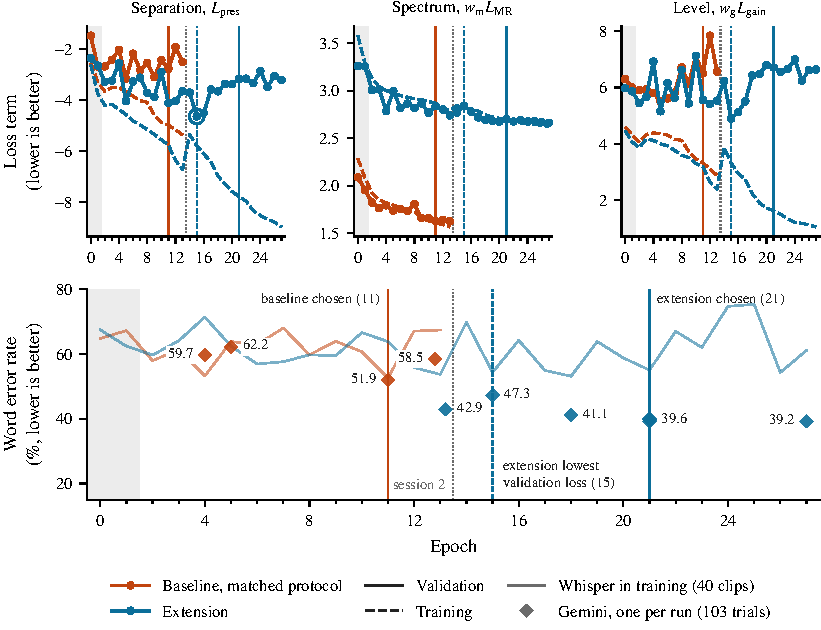
\includegraphics[width=\textwidth]{figures/training_curves.pdf}
  \caption{Training (dashed) and validation (solid) scores per epoch, counted from zero, for the baseline (orange) and the extension (blue), trained under the same protocol: the in-training Whisper check sets the learning rate and decides which epochs are kept. The baseline shown is epochs 0--13 of a 28-epoch run and is not yet judged; it is not the earlier baseline run that gives epoch 6 in the results tables. Top: the three weighted terms of the target-present loss, the first bracket of \autoref{eq:total}, which add up to it (lower is better): separation $L_\textup{pres}$, spectrum $w_\textup{m} L_\textup{MR}$ and level $w_\textup{g} L_\textup{gain}$. Bottom: word error rate on the 103 validation trials with both speakers present (lower is better). Each diamond is one run of the live judge on the same audio, labelled with the mean of the runs at that epoch; the thin lines are the in-training Whisper \texttt{small.en} check on 40 validation clips. Shaded epochs fail the \SI{-10}{dB} silence bar in both runs. The solid vertical line marks the extension's chosen epoch, the dashed one its lowest validation loss (the sum of the three terms), and the grey dotted line where training resumed in a second session.}
  \label{fig:training_curves}
\end{figure}

  



 \section{Evaluation setup}
  \subsection{Listeners}
  \label{sec:transcription}

  \paragraph{Offline ASR model}
  \label{sec:offline_asr}
  The offline transcriber is the \texttt{faster-whisper} implementation \cite{faster_whisper} of the Whisper \cite{radford2023whisper} model, run with the \texttt{large-v3-turbo} checkpoint. This is Whisper large-v3 with its decoder pruned from 32 layers to 4 and then fine-tuned, giving 809\,M parameters against the 1{,}550\,M of large-v3 \cite{whisper_turbo}. The large Whisper variants are a common choice for scoring how intelligible generated and extracted speech is \cite{anastassiou2024seedtts,wang2025solospeech}. Decoding was greedy, with a single sampling temperature of zero and no conditioning on previously decoded text, so the same audio always produces the same transcript, and the language was fixed to English. The smaller \texttt{small.en} checkpoint (244\,M parameters) is used only inside the training loop, where it transcribes a validation sample every epoch to shortlist checkpoints and schedule the learning rate. Scoring the results with a different checkpoint means the extension is not judged by the same listener it was tuned against.


  \paragraph{Live judge}
  \label{sec:live_judge}
  The live listener is \texttt{gemini-3.7-flash} \cite{google2026geminilive}, which was connected to via the \texttt{google-generativeai} Python package through the Application Programming Interface (API). The judge, like the ASR model, does not separate anything. The Gemini model is prompted to transcribe the estimated audio from the extractor, and then transcribes what it is able to hear. The judge is held out and never appears in the training loop in any form. This includes training using the judge as a proxy objective, This is to ensure that the judge is not biased towards any particular extractor and represents a fair evaluation of the extractor's performance. The live model is the tool for which this work is being built for and so it's result is the most important with respect to the overall evaluation of the extractor. 

  The prompt used can be found in \autoref{app:prompt}. It is deliberately worded to avoid instructing the judge to guess or pick a speaker to prevent the judge acting on the extractor's behalf. Secondly, it does not instruct the judge to guess as this would be a form of hallucination, which is a metric that is being measured and thus should not be confounded by the prompt. Finally, since live models by default will return some kind of reponse, the judge is prompted to return a structured response of a status field alongside the transcript. The status field is used to indicate whether the judge heard speech or not, and if it did not hear speech, the transcript is left empty. This allows for a clear distinction for whether the model hallucinates as the status field can be used to determine whether the model heard speech or not.

  \paragraph{Speech gating} [TODO mention the VAD tool used which was the same in the dataset setup]
  \label{sec:speech_gate}
  During experiments, it was common for both transcription tools to invent words when handed audio containing no speech frequently which led to many false positives. To address this issue, a speech gate was implemented to filter out any audio that appeared not to have speech that essentially acts as a pre-filter for the transcription tools. This method was considered for four reasons: \textit{(i)} if the gate is applied to a mixture that contained speech and the gate determines that the estimated audio does not contain speech, then it is already an indication that the extractor has failed to extract the target speaker, \textit{(ii)} if the gate is applied to a mixture that does not contain speech and the gate determines that the estimated audio does contain speech, then it is already an indication that the extractor has hallucinated, \textit{(iii)} if the gate is applied to a mixture that does not contain speech and the gate determines that the estimated audio does not contain speech, then it is already an indication that the extractor has correctly determined that there is no speech, and \textit{(iv)} this method is a practical implementation in a real system thus has a natural application to the evaluation of the extractor. Therefore it covers all possible scenarios and is a practical solution to the problem of hallucination. This method is support by \cite{whisper_hallucination_2025} and is applied for both the ASR and live judge.
  

  \subsection{Latency measures}
  During the course of experiments, the latency of the different systems was measured to compare the implemented model against \textit{(i)} the latency specification for live transcription, and \textit{(ii)} the latency of established systems. There are two main components to consider: time to consume and time to process the audio. The first component considers the real-time factor (RTF). The RTF is the ratio of the time taken to process the audio to the length of the audio, and for a model to be able to keep up with real-time audio, the RTF must be less than 1. This is The second component considers the latency created by the architecture itself which cannot be improved by faster hardware. To produce the output frame for a given window, the model must first have received that entire window, and the final lookahead samples (if considered) of it have not yet arrived. This forces a delay of the processing of the window as per the \autoref{sec:stft}. For the model to be able to keep up with real-time audio, the RTF needs to be less than one, and secondly, the budget for processing a frame must be less than 200-300ms as a standard for live transcription. 
  Finally, before either timing figure is interpreted, a probe checks whether a system can stream at all. A real-time factor cannot distinguish a model that is merely slow from one that requires the entire utterance before it can produce anything. The probe replaces all audio after a time $T$ and measures how far the output \emph{before} $T$ moves: if changing the future changes what the model has already produced, then that output depends on audio which has not yet arrived, and the model cannot be streamed. For a strictly causal model the movement must be zero. The replacement is made at matched loudness so that the overall level of the input is preserved.


\chapter{Results}
\label{ch:results}

% CLAIM THIS SECTION MUST SUPPORT: judge and offline ASR agree on the ranking of
% systems but fail by opposite mechanisms. See the error composition below.

[TODO:] Highlight that the model still has capacity to learn more with more training data and more parameters. Just that we needed a proof of concept. Also need to maybe put CARTSE's results in here for reference on another dataset.

In the results section, all reference to the "floor" and "ceiling" systems are related to passing the full mixture audio and the clean target audio respectively to the listener. This means that for the floor system, the listener is hearing the unprocessed mixture of the target and interferer and simulates what a listener would hear if the system did nothing. The ceiling system is the best possible outcome, where there is perfect separation and the listener hears only the target audio. The floor and ceiling systems are not real systems, but rather reference points for the listener to compare against. 
\section{Content fidelity}
\label{sec:results_content}
The main metrics to consider for this project is the performance of our extractor system with respect to the content fidelity on a live system. The content fidelity metrics are used to measure how the live artificial intelligence system is able to interpret the audio after the extraction process. The end goal is for the extractor to isolate and process the target speaker's audio in such a way for there to be minimal loss of content fidelity. Secondly, since the live system is a black box, non-deterministic system, the stability of the interpretation of the audio is also important to consider. 
The sections to follow consider the content fidelity for both a live judge and an offline transcriber.

\subsection{The live judge - Gemini Live}
\label{sec:results_content_judge}
The live judge results are shown in \autoref{tab:content_judge}. These results are most indicative of the overall performance of the extractor system as the live judge is the end user of the extraction process. To better understand the variability of the live judge on the same audio, \autoref{fig:judge_runs} shows how the different systems changed in the LCF-WER metric across three independent runs.
\begin{table}[H]
\centering
\caption{Content recovered by Gemini Live. \texttt{gemini-3.7-flash}, audio in and text out. Each value is the average of 3 runs on the same 103 trials, and $\pm$ is the standard deviation of those three run scores. \autoref{fig:judge_runs} shows how much the runs differ. Lower is better in every column.}
\label{tab:content_judge}
\small
\begin{tabular}{@{}lccccc@{}}
\toprule
 & LCF-WER \lowerbetter & ICR@2 \lowerbetter & mean leak \lowerbetter & invented \lowerbetter & FR@2 \lowerbetter \\
system & (\%) & (\%) & (\%) & /trial & (\%) \\
\midrule
Floor  & 62.94\,$\pm$\,0.37 & 75.73\,$\pm$\,0.00 & 63.90\,$\pm$\,0.65 & 1.27\,$\pm$\,0.03 & 30.7\,$\pm$\,3.1 \\
Baseline & 55.18\,$\pm$\,3.22 & 61.49\,$\pm$\,4.38 & 48.62\,$\pm$\,3.27 & 1.91\,$\pm$\,0.13 & 41.7\,$\pm$\,3.4 \\
Extension & 39.59\,$\pm$\,0.34 & 33.66\,$\pm$\,2.02 & 23.08\,$\pm$\,0.97 & 2.20\,$\pm$\,0.11 & 46.9\,$\pm$\,2.0 \\
WeSep & \textbf{25.80}\,$\pm$\,0.56 & \textbf{25.24}\,$\pm$\,0.97 & \textbf{13.04}\,$\pm$\,0.32 & \textbf{1.80}\,$\pm$\,0.02 & \textbf{38.6}\,$\pm$\,2.3 \\
Ceiling & 1.19\,$\pm$\,0.18 & 0.00\,$\pm$\,0.00 & 0.00\,$\pm$\,0.00 & 0.22\,$\pm$\,0.03 & 0.3\,$\pm$\,0.6 \\
\bottomrule
\end{tabular}
\end{table}

\begin{figure}[H]
\centering
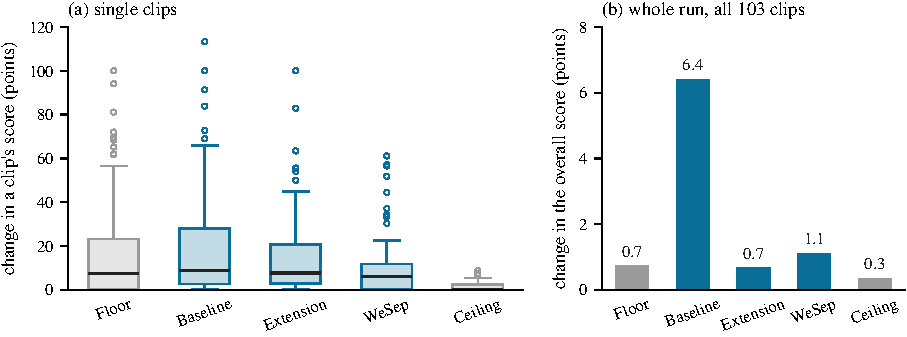
\includegraphics[width=\textwidth]{figures/judge_run_variation.pdf}
\caption{How much Gemini Live's LCF-WER changed across the three runs in \autoref{tab:content_judge}, where change is the highest of the three run scores minus the lowest. (a) Is the box plot showing how the change varies per clip over the averaged runs. A clip's score can pass 100\,\% and can occur when Gemini adds words through hallucination or including interfering speech. (b) Change in the overall score over all 103 clips. Floor and ceiling (grey) are reference points.}
\label{fig:judge_runs}
\end{figure}

The first comparison to be made is between the baseline and the floor. The baseline improves the LCF-WER by 7.76 points, which is a 12.3\,\% relative improvement over the floor. However, the baseline system evidently has extreme variation across the average performance over the three runs. The standard deviation of the LCF-WER is 3.22 points. There is a decisive improvement however in the baseline model's performance over the floor with regard to including an interfering speaker's content, as the average percentage of interfering words included in the output is 14.24 points lower than the floor. However, this came at a trade-off with the number of hallucinated words. Compared against the floor, the baseline system has fabricated/invented more words on average per trial as seen in the table. Finally, the baseline system also more frequently fabricates indicated by FR@2. Therefore, not only is the baseline system resulting in more words in a trial being fabricated (which is indicative of high degrees of artefacts), but it is also more likely on a random trial to fabricate words than the just passing the raw mixture audio. 

Overall, the baseline system is a clear improvement over the floor, which is indicative that the extractor has begun to find a signal in the mixture that is associated with the target speaker. The encouraging results can be seen when comparing the extension against the baseline and WeSep. WeSep acts as a benchmark for the best case scenario of what the BSRNN architecture can achieve from an extraction point of view although the WeSep model is both non-causal and cannot be used in a live system if there are latency concerns. For the extension, the inclusion of the pretrained ECAPA speaker encoder and passing the enrolment audio in parts instead of a single embedding has markedly improved the performance of the extractor. The LCF-WER has improved by 15.59 points over the baseline, which is a 28.3\,\% relative improvement. However, the most encouraging part of the results is how the extension has both reduced the number of leaked words per trial and the frequency of leakge by substantial amounts. The improvement can be attributed to the speaker specific information being passed to the extractor through the ECAPA speaker encoder. An interesting trade-off however is that the extension has increased the number of invented words per trial and the frequency of invention. This is indicative of the highly aggressive nature of the extractor, which was designed to mask out the interfering speaker's content however as a result, the masking can leave gaps or artefacts in the output which the live judge then interprets as words. 

To get a better idea of how stable the live judge is on the same audio, \autoref{fig:judge_runs} demonstrates how the LCF-WER changed across the three independent runs but measured per clip instead of the overall average. The idea is to gain a better understanding of how the standard deviation of the LCF-WER is distributed across the clips. The first observation is the confirmation of the extreme variability of the live judge when passed extracted audio by the baseline. In fact, the baseline has worse variability than the floor and the highest average in change of performance between the three runs. A very encouraging result is that the extension seems to have the best stability even when compared to WeSep. On single clips, there are outlier performance changes of up to 100 points (when one run results in 100 more errors than another run), these outliers could be incredibly difficult cases that are not indicative of the overall performance of the system. However, as seen in the bar plot, the extension on average has the smallest changes in overall performance across the three runs.
\subsection{The offline transcriber}
\label{sec:results_content_asr}
The offline transcriber serves to demonstrate how the extractor system performs on a standard transcription tool. The results are shown in \autoref{tab:content_asr}. The offline transcription system seems like a natural alternative to the live system whilst building the architecture as the live systems make use of paid APIs and are not open source. A researcher might thus be tempted to optimise for the offline transcriber and then hope that the improvements translate to the live system. 
\begin{table}[H]
\centering
\caption{Content recovered by the offline transcriber,
\texttt{faster-whisper small.en}. Lower is better in every column.}
\label{tab:content_asr}
\begin{tabular}{@{}lccccc@{}}
\toprule
 & WER \lowerbetter & ICR@2 \lowerbetter & mean leak \lowerbetter & invented \lowerbetter & FR@2 \lowerbetter \\
system & (\%) & (\%) & (\%) & /trial & (\%) \\
\midrule
Floor & 65.22 & 66.99 & 51.30 & 2.61 & 57.28 \\
Baseline & 59.52 & 50.49 & 34.58 & 3.08 & 68.00 \\
Extension & 56.72 & 32.04 & 15.76 & 3.61 & 76.24 \\
WeSep    & \textbf{34.60} & \textbf{15.53} & \textbf{9.02} & 3.03 & 73.79 \\
Ceiling  & 5.85 & 0.00 & 0.00 & 0.88 & 19.42 \\
\bottomrule
\end{tabular}
\end{table}


% CLAIMS THIS SECTION MUST SUPPORT:
%  (a) The offline ASR deletes MORE on the baseline's audio while the judge
%      deletes LESS (9.28 -> 12.60 against 5.97 -> 3.43). Same total by opposite
%      routes. This inverts the expectation that the ASR tolerates artefacts:
%      measured, the ASR is the brittle listener.
%  (b) WeSep wins by silencing the interferer, NOT by preserving the target.
%      Judge insertions fall 26.22 -> 8.99 (those words were the other speaker)
%      while deletions RISE to 6.78, worse than the baseline's 3.43 and worse
%      than doing nothing. LCF-WER on two-speaker mixtures is therefore
%      dominated by interferer suppression, and a system can lose target words
%      while halving the score. State this wherever LCF-WER is quoted.
\section{Error composition}
\label{sec:results_errors}
The LCF-WER metric is a combination of three different types of errors to form the word error rate: substitution, deletion and insertion. The metric is useful for breaking down the weaknesses of the extractor system and to better understand how the system is introducing error. For example, a system with high deletions is indicative of over suppression of the target speaker's content, a system with high insertions is indicative of hallucination or leakage, and finally a system with high substitutions is indicative of misinterpretation of the target speaker's content. The error composition for both the live judge and the offline transcriber are shown in \autoref{tab:error_split}.
\begin{table}[H]
\centering
\caption{Substitution (S), deletion (D) and insertion (I) rates for each listener. Lower is better.}
\label{tab:error_split}
\begin{tabular}{@{}lcccccc@{}}
\toprule
& \multicolumn{3}{c}{Gemini Live} & \multicolumn{3}{c}{Offline ASR} \\
\cmidrule(lr){2-4}\cmidrule(lr){5-7}
system & $S$ \lowerbetter & $D$ \lowerbetter & $I$ \lowerbetter & $S$ \lowerbetter & $D$ \lowerbetter & $I$ \lowerbetter \\
\midrule
Floor    & 29.22 & 5.97 & 28.08 & 32.89 & 9.28  & 23.05 \\
Baseline & 25.64 & 3.00 & 26.95 & 28.20 & 11.79 & 19.53 \\
Extension & 16.96 & 9.44 & 13.19 & 24.07 & 16.30 & 16.36 \\
WeSep    & 10.62 & 6.78 & 8.99  & 18.51 & 8.91  & 7.19 \\
Ceiling  & 0.87  & 0.15 & 0.03  & 3.43  & 0.67  & 1.75 \\
\bottomrule
\end{tabular}
\end{table}

The first observation is related to the live judge and how it performs when given a raw mixture. As expected, the floor system has a high insertion rate of 28.08\,\% which is indicative of the interfering speaker's content being included in the output and then a high substitution rate of 29.22\,\% which is indicative of the live judge misinterpreting the target speaker's content. The deletion rate is comparatively much lower at 5.97\,\% but not 0\,\%. This means that even with no masking, the live system can miss some of the target speaker's content. 


% CLAIMS THIS SECTION MUST SUPPORT:
%  (a) No signal-domain measure predicts what the listener recovered: SI-SDR
%      improved by 1.99 dB while 30 % of trials got WORSE on content, and delta-SDR
%      explains only ~4 % of the variance in content outcome.
%  (b) SAR is the single column the baseline wins, and it is the one that says
%      why: WeSep removes 7.1 dB more interferer and pays for it in artefact.
%  (c) NEVER quote delta-SAR. The floor's +30 dB is an artefact of the cap, not a
%      measurement, so any improvement against it is meaningless. Absolute SAR
%      of +10.34 dB means roughly 9 % of the output energy was invented.
\section{Signal-domain separation}
\label{sec:results_signal}
A key part of the training process is to introduce the idea of separation. The three kinds considered in this project is separation of the target from the background noise (distortion), interference from other speakers (interference) and finally from artefacts introduced by the extractor system (artefact). The signal-domain separation results are shown in \autoref{tab:signal}. These metrics highlight what the extractor system is doing in the signal domain and can best be used to understand the trade-offs between the different types of separation. A note about the values in the table: SAR for the floor and ceiling are both at +30 dB, as since these systems do not contain a model there can be no artefacts introduced. 
\begin{table}[H]
\centering
\caption{Signal-domain decomposition, in \si{\decibel}; higher is better. The ceiling reaches \SI{+30}{\decibel} by construction, where the cap created by the denominator floor $\tau = 10^{-3}$, and is not a measurement. Reference Section~\ref{sec:results_errors} for more details.}
\label{tab:signal}
\begin{tabular}{@{}lccc@{}}
\toprule
system & SDR \higherbetter & SIR \higherbetter & SAR \higherbetter \\
\midrule
Floor & $-1.12$ & $-1.12$ & $+30.00$ \\
Baseline & $+1.29$ & $+3.66$ & $+11.11$ \\
Extension & $+2.29$ & $+9.17$ & $+6.28$ \\
WeSep   & $+4.68$ & $+10.34$ & $+8.26$ \\
Ceiling  & $+30.00$ & $+30.00$ & $+30.00$ \\
\bottomrule
\end{tabular}
\end{table}
The most noticeable observation is that the extension has significantly improved the SIR metric over the baseline, and is comparable to the WeSep model. The gap in performance between the extension and WeSep therefore seems to lie in the SAR and SDR metric. Therefore when considering how to improve the extension, the next iteration should potentially target mechanisms that reduce the artefacts introduced by the extractor system. Interestingly, the baseline has a highest model SAR metric. However this should not be attributed to the model being better at reducing artefacts, but rather due to the simplistic nature of the model design. The baseline model is not as aggressive in masking out the interfering speaker's content, and therefore does not introduce as many artefacts into the output. 

% CLAIMS THIS SECTION MUST SUPPORT:
%  (a) THE DIVERGENCE. The baseline improved content by 6.1 points while OVRL
%      FELL from 2.497 to 2.237. A human listener would say it damaged the audio;
%      the listener recovered more of the words. A conventional perceptual metric
%      would have rejected a system that measurably helps the task.
%  (b) SIG fell 0.72 while BAK rose 0.24 -- three times as far -- confirming from
%      an independent instrument that artefact added outweighs interference
%      removed. This is the perceptual analogue of the SIR/SAR split.
%  (c) P808 is flat at +0.02. The metric the REAL-TSE organisers switched TO is
%      nearly blind to what this model does, while OVRL, the one that was gamed,
%      moves.
\section{Perceptual quality}
\label{sec:results_perceptual}
The perceptual quality metrics are used to indicate that extraction audio that sounds good to a proxy of a human listener does not necessarily translate to better content fidelity. The perceptual quality metrics are shown in \autoref{tab:dnsmos}. 
\begin{table}[H]
\centering
\caption{DNSMOS, personalised model. All scores are between 1 and 5 where the higher the score, the better.}
\label{tab:dnsmos}
\begin{tabular}{@{}lcccc@{}}
\toprule
system & P808 \higherbetter & SIG \higherbetter & BAK \higherbetter & OVRL \higherbetter \\
\midrule
Floor & 2.913 & 4.090 & 2.031 & 2.497 \\
Baseline  & 2.955 & 3.233 & 2.286 & 2.183 \\
Extension & \textbf{3.030} & 2.957 & \textbf{3.045} & 2.306 \\
WeSep   & 3.010 & \textbf{3.450} & 2.640 & \textbf{2.510} \\
Ceiling  & 3.550 & 4.175 & 3.592 & 3.429 \\
\bottomrule
\end{tabular}
\end{table}

First considering P808 in isolation, the extension seemingly has a similar, if not slightly better, overall quality score than WeSep. Therefore by the one perceptual quality metric our extension produces audio that is more pleasing to a human listener (by the P808 model standards) than the WeSep model. However, when considering the other three metrics that form part of the second perceptual quality metric, the WeSep model has a better SIG and OVRL score than the extension. However, something fascinating to note is how the extension scores lower than the floor for both the SIG and OVRL metrics, and yet as seen in the content fidelity results, the extension has improved the content fidelity over the floor by a significant margin. This is an interesting observation as it demonstrates that the perceptual quality metrics are not good indicators for the purposes of this research project, which is to improve the content fidelity of the target speaker's audio. The metric in itself is subjective to the actual perceptual system and does not provide indication that what sounds good to a human listener is necessarily better for the content fidelity of the target speaker's audio.

% CLAIMS THIS SECTION MUST SUPPORT:
%  (a) The causality probe must be reported BEFORE the timings are interpreted.
%      WeSep moved its output before the cut by 1.12e-02 under a scale-matched
%      perturbation, against our own model's 1.68e-08. Every output frame depends
%      on the whole clip, so its RTF is academic: a model that needs the entire
%      utterance cannot stream at any speed.
%  (b) Mechanism: `causal: true` is not a false claim, it is narrower than it
%      reads. The separator's RNNs are causal, but SubbandNorm normalises over all
%      channels AND all time frames -- a whole-utterance statistic computed before
%      the causal separator sees anything.
%  (c) No WeSep chunk finishes inside its own 80 ms, so the backlog grows without
%      bound. Two causes: 27.2 M parameters in the timed forward against our
%      7.19 M, and the 5 s enrolment re-embedded through a full speaker encoder on
%      every chunk against our cheap TF-Map cue. The protocol is matched; the cost
%      is not.
\section{Latency and throughput}
\label{sec:results_latency}

\begin{table}[H]
\centering
\caption{Latency and throughput over 2{,}250 chunks of \SI{80}{\milli\second} on CPU (i5-1135G7, 4 threads), except where marked. The requirement is $\textup{RTF} < 1$ \emph{and} latency within \SI{200}{}--\SI{300}{\milli\second}; the first is the binding constraint, because a chunk that finishes inside its own duration meets the latency budget automatically. Every figure is an \emph{estimate}, not a streaming measurement: chunks are processed independently with no carried state, which is worth 10--20\,\% either way.}
\label{tab:latency}
\small
\begin{tabular}{@{}lccccc@{}}
\toprule
 & \multicolumn{2}{c}{RTF \lowerbetter} & \multicolumn{2}{c}{latency (\si{\milli\second}) \lowerbetter} & meets \\
\cmidrule(lr){2-3}\cmidrule(lr){4-5}
system & mean & p99 & mean & p99 & budget \\
\midrule
Baseline      & 0.783 & 1.095 & 182.6 & 207.6 & mean only \\
Extension & 0.536 & 0.751 & 162.9 & 180.1 & yes \\
WeSep & 2.854 & 5.300 & 348.3 & 544.0 & no$^\ddagger$ \\
\bottomrule
\end{tabular}

\vspace{0.5em}
{\footnotesize $^\dagger$ Timed over 500 chunks, where every other row uses 2{,}250. The shorter run reads systematically faster, so this row is \emph{not} comparable with the rest of the table and its apparent win is an artefact of the protocol. Re-timing it is outstanding.\\
$^\ddagger$ And cannot stream at all, independently of its throughput. See the causality result above.}
\end{table}

The extension needs about \SI{67}{\milli\second} to process each \SI{80}{\milli\second} of audio, so on a typical chunk it finishes with roughly \SI{13}{\milli\second} to spare and holds pace with a live stream. The delay a listener would experience averages \SI{187}{\milli\second}: the \SI{80}{\milli\second} of audio that must arrive before the chunk can be processed, the \SI{40}{\milli\second} of lookahead the architecture requires, and the compute itself. The slowest one percent of chunks reach \SI{222}{\milli\second}. Both figures sit inside the \SI{200}{}--\SI{300}{\milli\second} budget.

The worst chunks, however, do not keep up, and that is the constraint that binds. The slowest one percent take \SI{102}{\milli\second} to process \SI{80}{\milli\second} of audio, so during those chunks work arrives faster than it is cleared and a backlog forms. The delays quoted above assume no queue; under a burst of slow chunks the true delay exceeds them by whatever backlog has built up, which means \SI{222}{\milli\second} is a floor rather than a worst case. The 9{,}955-trial model behaves the same way (p99 1.095). Only the 4{,}976-trial row clears the deadline at the 99th percentile, and that row was timed under a protocol which flatters it.

The extension is not slower than the model it extends. Compared like for like at 2{,}250 chunks it costs 7\,\% more compute per chunk (0.783 against 0.839) and \SI{4.5}{\milli\second} more delay, but the two share an architecture and a parameter count of 7{,}189{,}644: the mask-structure term acts on the training objective and leaves the network untouched, so the true difference is zero by construction and the gap measures run-to-run variation on a laptop CPU. It must not be read as a cost of the extension.

All of these timings come from a four-thread laptop CPU of 2021 vintage, whereas the deployment assumption is server-class hardware. They are therefore a conservative bound and not a projection of deployed performance; a GPU timing remains outstanding.


% TODO: write out as prose. The four that must appear:
%  1. Signal and perceptual rows are listener-independent; only content has a
%     listener at all.
%  2. `sir0_val` is symmetric by construction and therefore harder than
%     `eval_public` -- 7.8 points apart on the floor alone. Which set defines the
%     benchmark is still undecided.
%  3. Every judge figure is an aggregate. Per-trial judge numbers carry up to 16
%     points of noise (SEM approx. 0.5 over n = 103), so no per-trial judge
%     comparison is meaningful.
%  4. No figure here is comparable to any published REAL-TSE result: different
%     data, different metric, different protocol.

\section{Conclusion}
\label{sec:conclusion}

\subsection{Key findings}
% TODO
\subsection{Limitations}
The shortcomings of the work are the extractor's weakness in removing interfering speech, whilst simultaneously not introducing artefacts that get misinterpreted by the downstream model as target speech.

\subsection{Future work}
The structure and nature of the approach formulated in this work allows for a number of future directions to be explored.   
\begin{itemize} 
      \item \textbf{Streaming architecture.} The LSTM layers of the extractor could be replaced with state space layers. A state space layer is a recurrent layer whose updates are linear, which allows for parallel training while still running frame by frame. SA-Mamba \cite{liu2026samamba} applies this idea within a band-split, dual-path design similar to the one in this work, and conditions the state space layers on the target speaker. It placed second in the online track of the REAL-TSE challenge, while its report describes training on simulated mixtures only, and the
  organisers attribute most of the gains of the top systems to their data \cite{wang2026realtse}. The architecture has not yet been used with a live speech model as the listener and secondly it did not have a training recipe built around one, as in this work. 
      \item \textbf{Training objective.} The current objective is a proxy for general extraction rather than for the downstream task. Weighting the leaked speech or the artefacts in the loss moved errors from one source to the other but did not lower the LCF-WER (\autoref{sec:results_metric}), so an objective closer to \emph{how} Gemini listens is still needed.
      \item \textbf{Removing interfering speech without artefacts.} As seen in the results, the extractor struggles with the trade-off between removing interfering speech and introducing artefacts. A likely reason is the aggressive masking, which can leave sharp transitions where the interfering speech was removed. The extractor could instead be trained to also extract the interfering speaker, so that it learns what to remove as well as what to keep.
      \item \textbf{Filling the gaps for Gemini.} Rather than leaving gaps where the interfering speech was removed, the extractor could fill them with a signal that Gemini ignores, such as low-level noise, leaving nothing for Gemini to fill with words. Gemini, during experimentation, was found to be robust to very low-level noise, but the idea is to make audio clips that are optimised to be ignored by the listener.
      \item \textbf{Adaption to real recordings.} Although fine-tuning to the live transcriber did not yield improvements, the extractor could be adapted to real recordings after training on simulated mixtures.
      \item \textbf{Learning the band plan.} No paper has yet justified the actual boundaries of the bands used in the band-split design. Learnable band positionings could find better boundaries for the extractor and could be conditioned on the target speaker. This will introduce another conditioning to the extractor, which by the extension in this work showed to be beneficial.
  \end{itemize}


% Bibliography
\phantomsection  % contents link lands on References, not the Conclusion
\bibliography{references}

% End matter
\clearpage
\appendix
\section{Evaluation protocol details}
\label{app:protocol}

\subsection{Prompt for live-model transcription}
\label{app:prompt}

\begin{verbatim}
Write down the words spoken in this audio, exactly as spoken.

If no words are audible, leave the transcript empty and set status to no_speech.
\end{verbatim}


\subsection{Pinned components of the measuring instrument}
\label{app:pinned}

% TODO: complete the judge row once selected. Every judge result must record
% the exact model identifier, the exact prompt, the input modality and the run
% date. Cross-date comparison is treated as valid; see decisions-m4.md 2026-09-07.

\begin{table}[H]
  \mytable
  \begin{tabularx}{\textwidth}{@{}lL@{}}
    \toprule
    Component & Identity \\
    \midrule
    Text normaliser        & \texttt{whisper-normalizer} 0.1.15, \texttt{EnglishTextNormalizer} \cite{whisper_normalizer,radford2023whisper} \\
    Baseline transcriber   & \texttt{faster-whisper} 1.2.1, \texttt{large-v3-turbo}, int8 quantisation, greedy decoding \cite{faster_whisper,radford2023whisper,whisper_turbo} \\
    In-loop transcriber    & \texttt{faster-whisper} 1.2.1, \texttt{small.en}, int8 quantisation, greedy decoding; training-time checkpoint shortlisting only \\
    Word error rate        & \texttt{jiwer} 4.0.0 \cite{jiwer} \\
    Stopword list          & \texttt{NLTK} English stopwords \cite{bird2009nltk}, snapshotted into the source tree so the list cannot change with a library upgrade \\
    Judge model            & \texttt{gemini-3.7-flash} \\
    Random seed            & 42 \\
    \bottomrule
  \end{tabularx}
  \caption{Components of the evaluation instrument, pinned by version. A change
           to any row invalidates comparison with numbers reported before it.}
  \label{tab:pinned}
\end{table}


\section{Room construction}
\label{app:rooms}
\label{sec:room_construction}

Each trial is rendered in its own simulated room rather than convolved with a
recorded impulse response, so that the acoustics are a controllable variable
rather than a property of whichever room happened to be recorded. Rooms are
rectangular (``shoebox'') and the impulse responses are generated by the
image-source method using \texttt{pyroomacoustics} 0.10.1
\cite{scheibler2018pyroomacoustics}.

For every trial the renderer draws the room's three dimensions, a reverberation
time, and independent positions for the microphone and the two talkers. Wall
absorption is not drawn directly: it is solved for from the requested
reverberation time and the room's surface area by the Sabine relation, and the
draw is rejected and retaken if the combination is not physically realisable.
Both talkers are placed in the same room and share the microphone, so the two
speech signals arrive with different but consistent room responses.

\begin{figure}[H]
  \centering
  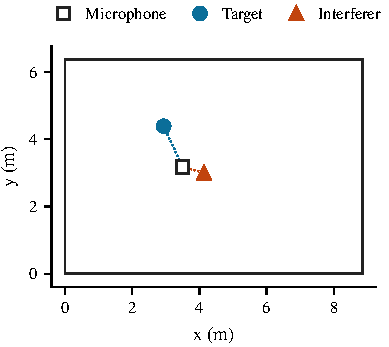
\includegraphics[width=0.4\textwidth]{figures/room_example_a.pdf}
  \caption{Plan view of the room rendered for trial \texttt{train-42-007495}. The room measures $8.85 \times 6.38 \times \SI{3.14}{\metre}$ (\SI{177}{\cubic\metre}) with a reverberation time of \SI{0.250}{\second}, for which the Sabine relation gives a wall absorption of \num{0.5479}. The microphone sits at $(3.50, 3.18, 1.28)$~m, the target at $(2.94, 4.39, 1.66)$~m and the interferer at $(4.14, 3.00, 1.57)$~m, placing them \SI{1.39}{\metre} and \SI{0.72}{\metre} from the microphone respectively.}
  \label{fig:room_a}
\end{figure}


\section{Construction parameters}
\label{app:params}

Every parameter below is drawn independently per trial from the stated distribution, except where a regime overrides it. Ranges written $[a, b]$ are sampled uniformly on that interval.

% xltabular, not table + tabularx: a float cannot break across pages, and this
% table is taller than one. The header repeats on every page it spans.
\begingroup
  \small
  \renewcommand{\arraystretch}{1.2}
  \begin{xltabular}{\textwidth}{@{}llL@{}}
    \toprule
    Parameter & Distribution & Meaning \\
    \midrule
    \endfirsthead
    \toprule
    Parameter & Distribution & Meaning \\
    \midrule
    \endhead
    \midrule
    \multicolumn{3}{r@{}}{\emph{Continued on the next page}} \\
    \endfoot
    \bottomrule
    \caption{Construction parameters and their sampling distributions.}
    \label{tab:params}
    \endlastfoot
    \multicolumn{3}{@{}l}{\emph{Trial layout}} \\
    Mixture length        & $[15.0, 20.0]$ s   & Duration of the rendered trial \\
    Overlap ratio         & $[0.0, 0.7]$       & Fraction of target speech with the interferer also talking \\
    Overlap tolerance     & $0.03$             & Accepted deviation from the requested overlap \\
    Target activity ratio & $[0.15, 0.78]$     & Fraction of the trial in which the target speaks \\
    Activity tolerance    & $0.1$              & Accepted deviation from the requested activity \\
    Utterances per source & $\le 6$            & Cap on how many utterances one recording may contribute \\
    \midrule
    \multicolumn{3}{@{}l}{\emph{Levels}} \\
    SIR                   & $[-5.0, 15.0]$ dB  & Target loudness relative to the interferer \\
    SNR                   & $[0.0, 20.0]$ dB   & Target loudness relative to the noise bed \\
    Target loudness       & $[-33.0, -25.0]$ LUFS & Absolute level of the target, BS.1770 integrated \cite{itu2015bs1770} \\
    Clip ceiling          & $0.95$             & Peak after which the whole trial is rescaled together \\
    \midrule
    \multicolumn{3}{@{}l}{\emph{Room}} \\
    $T_{60}$              & $[0.25, 0.6]$ s    & Reverberation time \\
    Room length, width    & $[5.0, 10.0]$ m    & Floor plan \\
    Room height           & $[3.0, 4.0]$ m     & \\
    Source distance       & $[0.1, 2.0]$ m     & Talker to microphone \\
    Source height         & $[0.9, 1.8]$ m     & Talker, seated to standing \\
    Microphone height     & $[0.9, 1.8]$ m     & \\
    Early reflections     & $50$ ms            & Cutoff separating early echoes from the late tail \\
    \midrule
    \multicolumn{3}{@{}l}{\emph{Enrolment}} \\
    Enrolment length      & $5.0$ s            & Single clip, levelled, carrying no room \\
    EQ augmentation       & $p = 0.5$          & Three peaking biquads, log-uniform \SIrange{120}{6400}{\hertz}, $\pm$\SI{6}{\decibel}, $Q = 1.0$, RMS restored \\
    \midrule
    \multicolumn{3}{@{}l}{\emph{Speaker pairing}} \\
    Same-gender fraction  & $0.5$              & Proportion of trials whose two talkers share a gender \\
    \midrule
    \multicolumn{3}{@{}l}{\emph{Speech detection} \cite{silero2021vad}} \\
    Silence threshold     & $250$ ms           & Pause length after which a talker counts as stopped; \textbf{this defines overlap} \\
    Speech probability    & $0.5$              & Frame-level threshold \\
    Minimum speech        & $100$ ms           & Shortest run counted as speech \\
    Speech padding        & $30$ ms            & Added either side of a detected run \\
    Noise-bed rejection   & $0.5$ s            & Longest run of detected speech tolerated in a WHAM! clip \\
    \midrule
    \multicolumn{3}{@{}l}{\emph{Regimes}} \\
    Regime weights        & $0.6$ / $0.4$      & Proportion of trials drawn as \texttt{base} / \texttt{hard} \\
    \texttt{base} SIR     & $[0.0, 12.0]$ dB   & Regime override \\
    \texttt{base} SNR     & $[8.0, 20.0]$ dB   & Regime override \\
    \texttt{base} activity & $[0.45, 0.78]$    & Regime override \\
    \texttt{base} $T_{60}$ & $[0.25, 0.5]$ s   & Regime override \\
  \end{xltabular}
\endgroup



\end{document}

